\section{Thiết kế giao diện}
\subsection{Landing Page}
\begin{figure}[H]
    \centering
    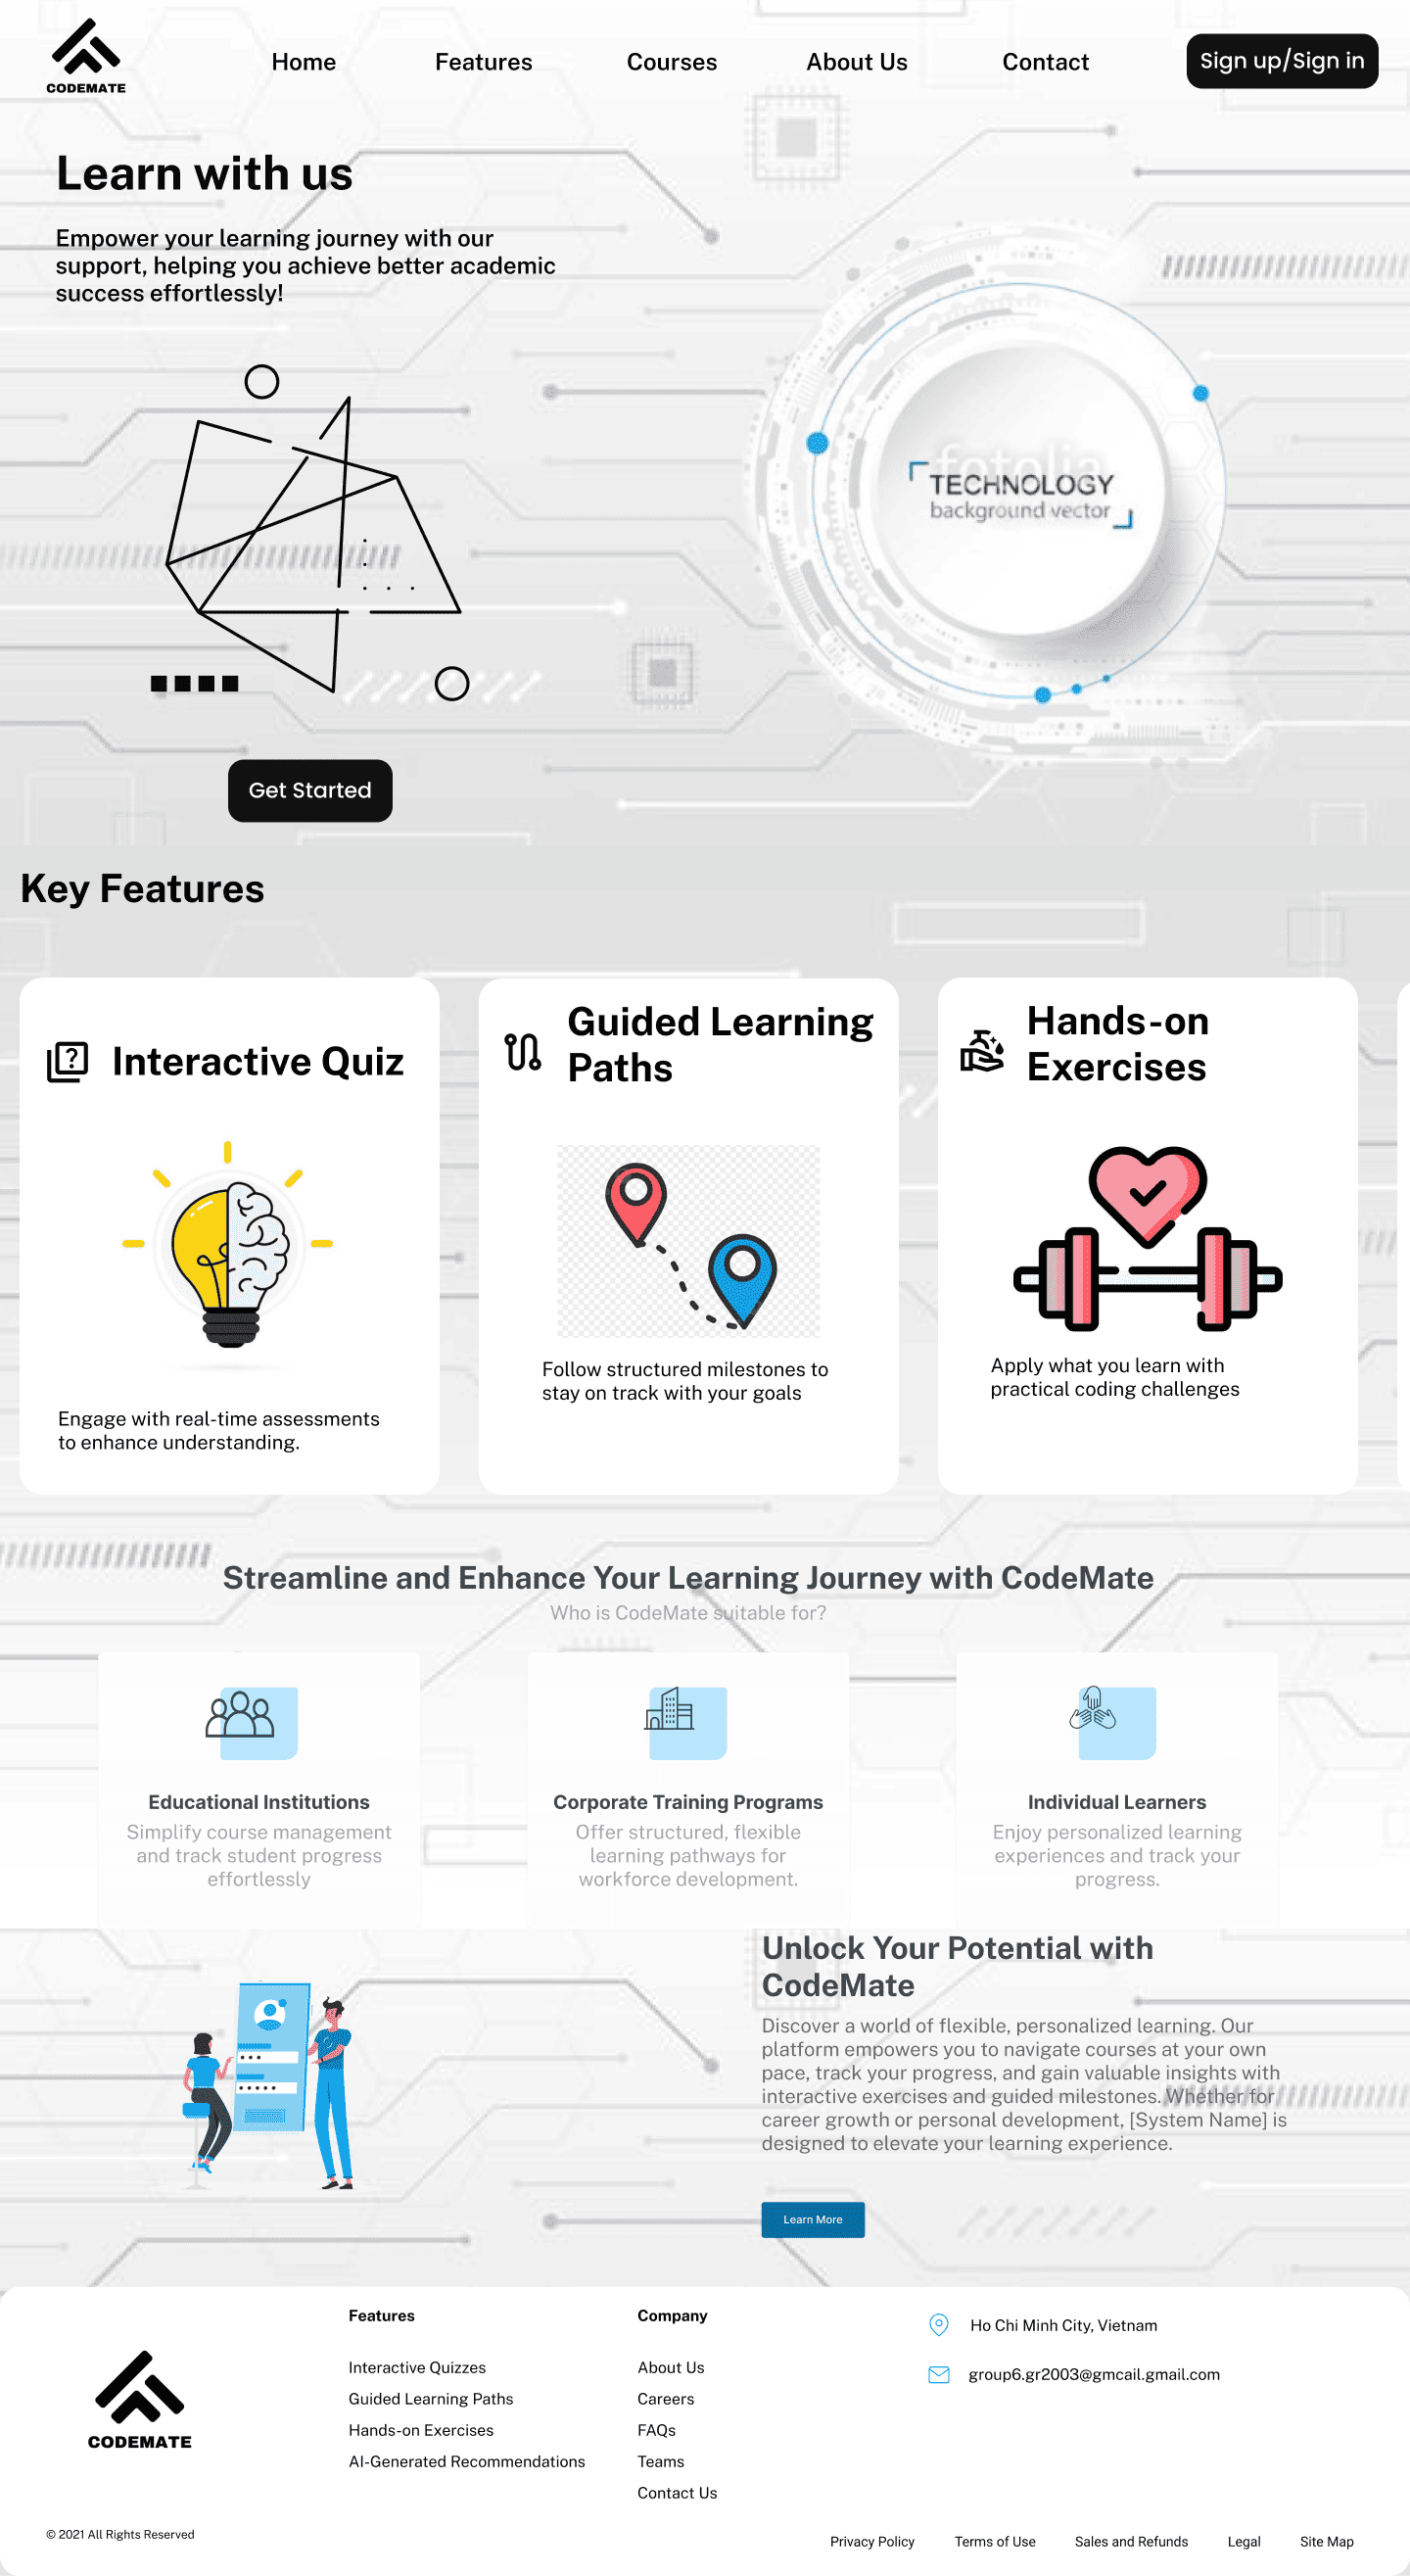
\includegraphics[width=0.7\linewidth]{Images/figmaDesign/Landing Page.png}
    \caption{Landing Page}
    \label{fig:enter-label}
\end{figure}
Landing Page mô tả tổng quát về website hỗ trợ học tập \textbf{\textit{CODEMATE}}.
\subsection{Authentication}
\subsubsection{Log In Screen}
\begin{figure}[H]
    \centering
    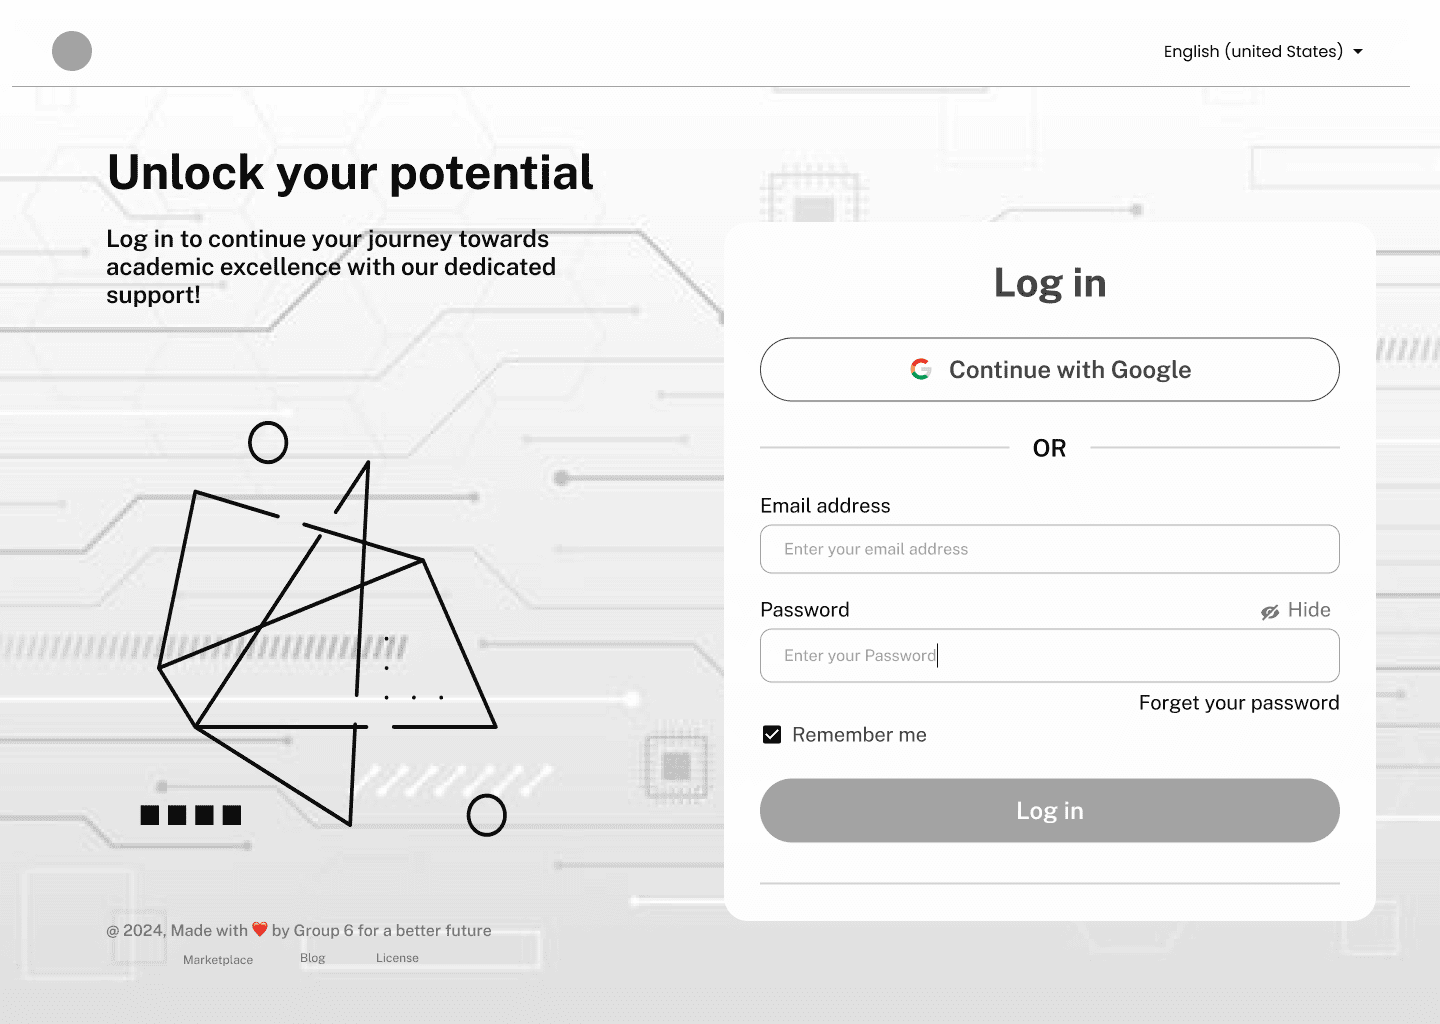
\includegraphics[width=0.7\linewidth]{Images/figmaDesign/Sign In Screen.png}
    \caption{Log In Screen}
    \label{fig:enter-label}
\end{figure}
Trang đăng nhập hệ thống, cho phép người dùng đăng nhập vào hệ thống bằng Email của mình hoặc qua phương thức đăng nhập bằng bên thứ ba \textbf{\textit{(Google)}}. Hệ thống sẽ nhận diện tên miền riêng của Email để xác định tính xác thực của Email trường Đại học do người dùng cung cấp. Nếu người dùng không dùng Email do trường Đại học cung cấp, sẽ không thể truy cập vào hệ thống. Ngoài ra, role của người dùng cũng sẽ được hệ thống phân loại dựa vào Email Address của người dùng và cơ sở dữ liệu của trường Đại học cung cấp cho hệ thống. 
\subsubsection{Forgot Password Screen}
\begin{figure}[H]
    \centering
    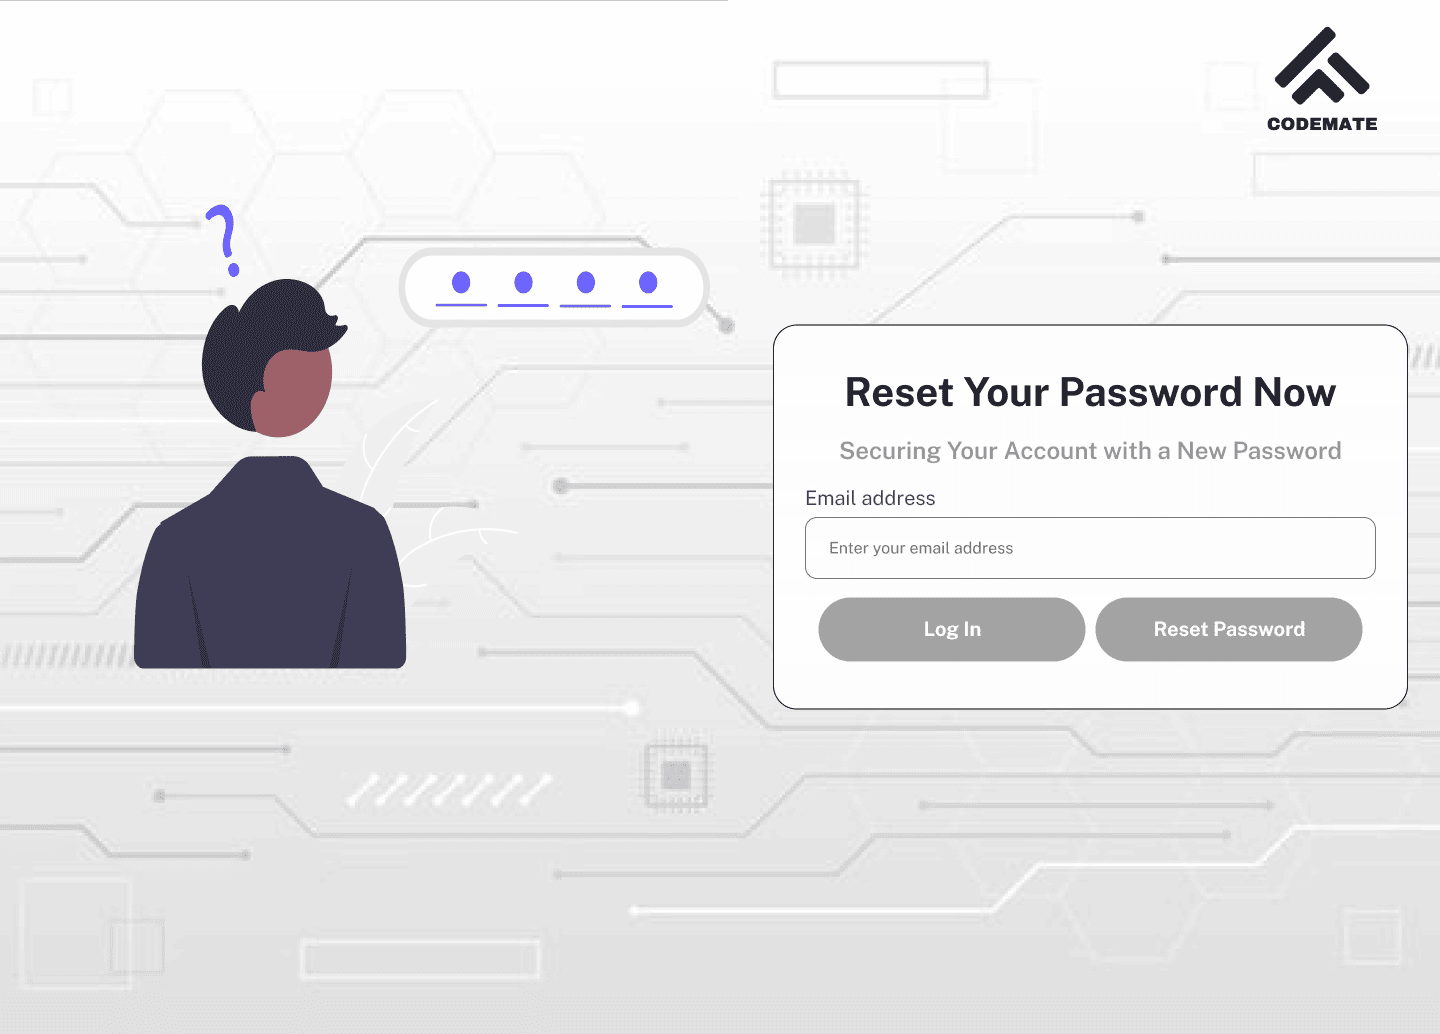
\includegraphics[width=0.7\linewidth]{Images/figmaDesign/Forgot Password Screen.png}
    \caption{Forgot Password Screen}
    \label{fig:enter-label}
\end{figure}
\subsubsection{Reset Password Screen}
\begin{figure}[H]
    \centering
    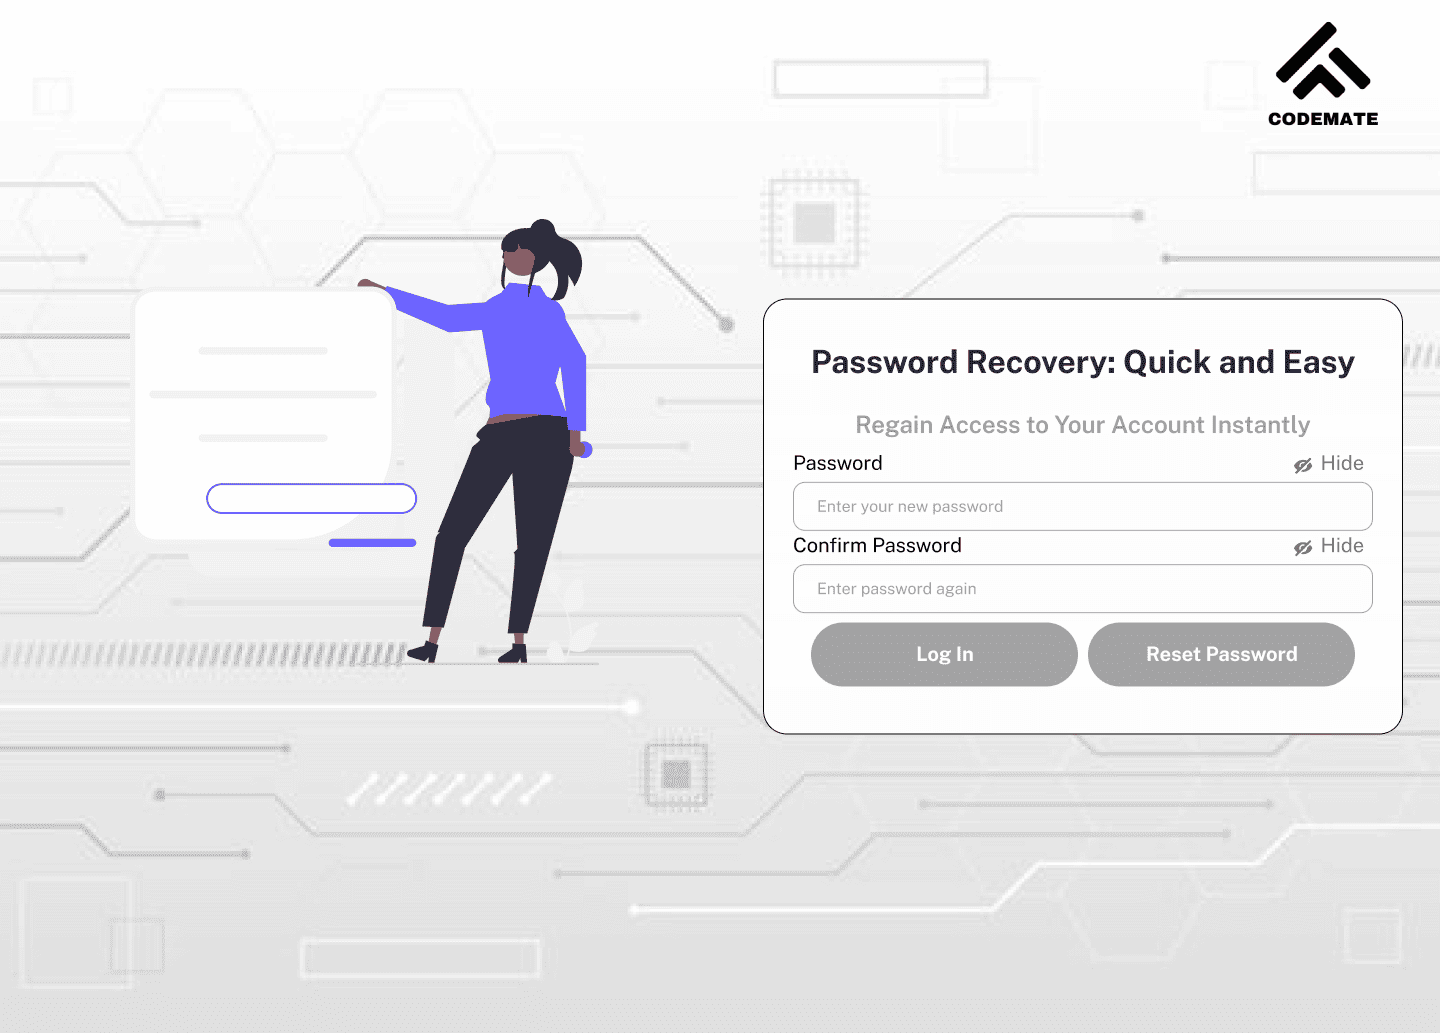
\includegraphics[width=0.7\linewidth]{Images/figmaDesign/Reset Password Screen.png}
    \caption{Reset Password Screen}
    \label{fig:enter-label}
\end{figure}
Các trang \textbf{\textit{"Forgot Password"}} và \textbf{\textit{"Reset Password"}} hỗ trợ người dùng trong trường hợp quên mật khẩu truy cập vào hệ thống và muốn lấy lại mật khẩu của mình thông qua địa chỉ Email. 
\subsection{Course Management (Student)}
\subsubsection{Courses List Screen}
\begin{figure}[H]
    \centering
    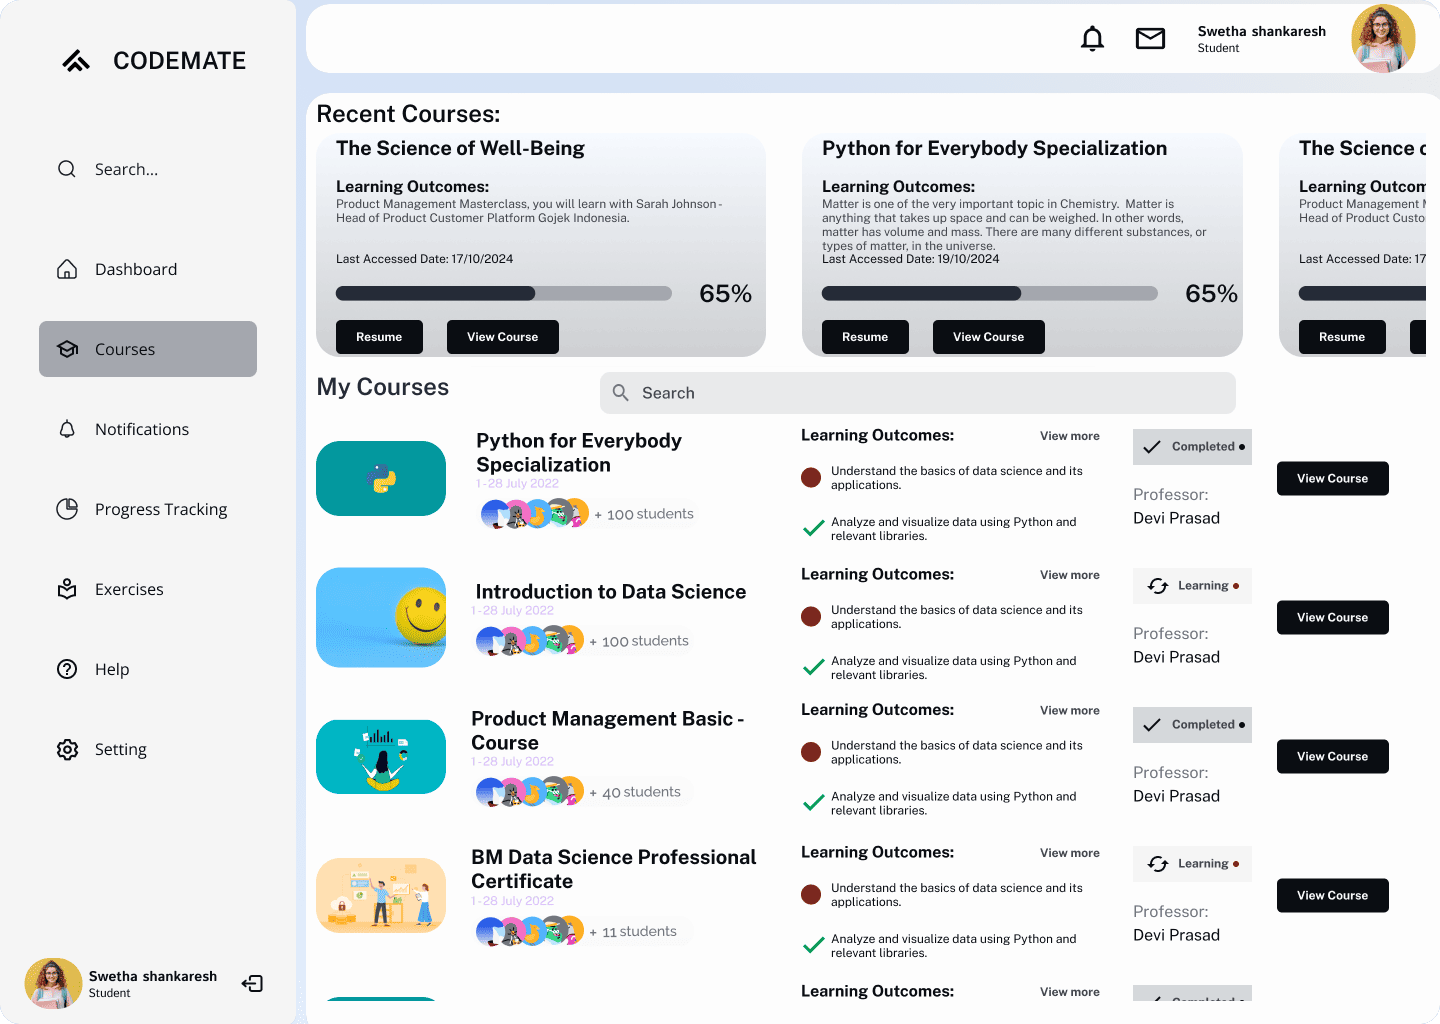
\includegraphics[width=0.7\linewidth]{Images/figmaDesign/Courses List Page.png}
    \caption{Courses List Screen}
    \label{fig:enter-label}
\end{figure}
Trang danh sách khóa học, hiển thị danh sách các khóa học mà sinh viên đã đăng ký tại học kỳ đó. Đặc biệt là các khóa học liên quan đến lĩnh vực \textbf{\textit{"Khoa học máy tính"}}. Sinh viên có thể xem các khóa học mình đã và đang học hoặc các khóa học truy cập gần đây. Mỗi khóa học hiển thị các thông tin như: \textbf{\textit{Tên khóa học, Tên giảng viên, Thời gian bắt đầu, Thời gian kết thúc, Đầu ra môn học}} và tác vụ \textbf{\textit{"Xem chi tiết khóa học"}}.
\begin{figure}[H]
    \centering
    
\includegraphics[width=0.7\linewidth]{Images/figmaDesign/Modal Learning Outcomes.png}
    \caption{Modal Learning Outcomes}
    \label{fig:enter-label}
\end{figure}
Sinh viên có thể xem chi tiết \textbf{\textit{"Đầu ra môn học"}} bằng nút \textbf{\textit{"View more"}}
\subsubsection{Detailed Course Screen}
Trang thông tin chi tiết khóa học, field Description, cho phép sinh viên xem mô tả \textbf{\textit{"Đầu ra môn học"}} do giảng viên cung cấp. Ngoài ra, các thông tin của khóa học như:\textbf{\textit{Tên môn học, Phần trăm hoàn thành hiện tại khóa học của sinh viên, Label trạng thái môn học, Số unit của khóa học, Tên giảng viên}} được hiển thị chung ở một component. Mỗi khóa học sẽ có 3 fields hỗ trợ cho các thông tin: \textbf{\textit{Description, Lessons, Exercises}}. 
\begin{figure}[H]
    \centering
    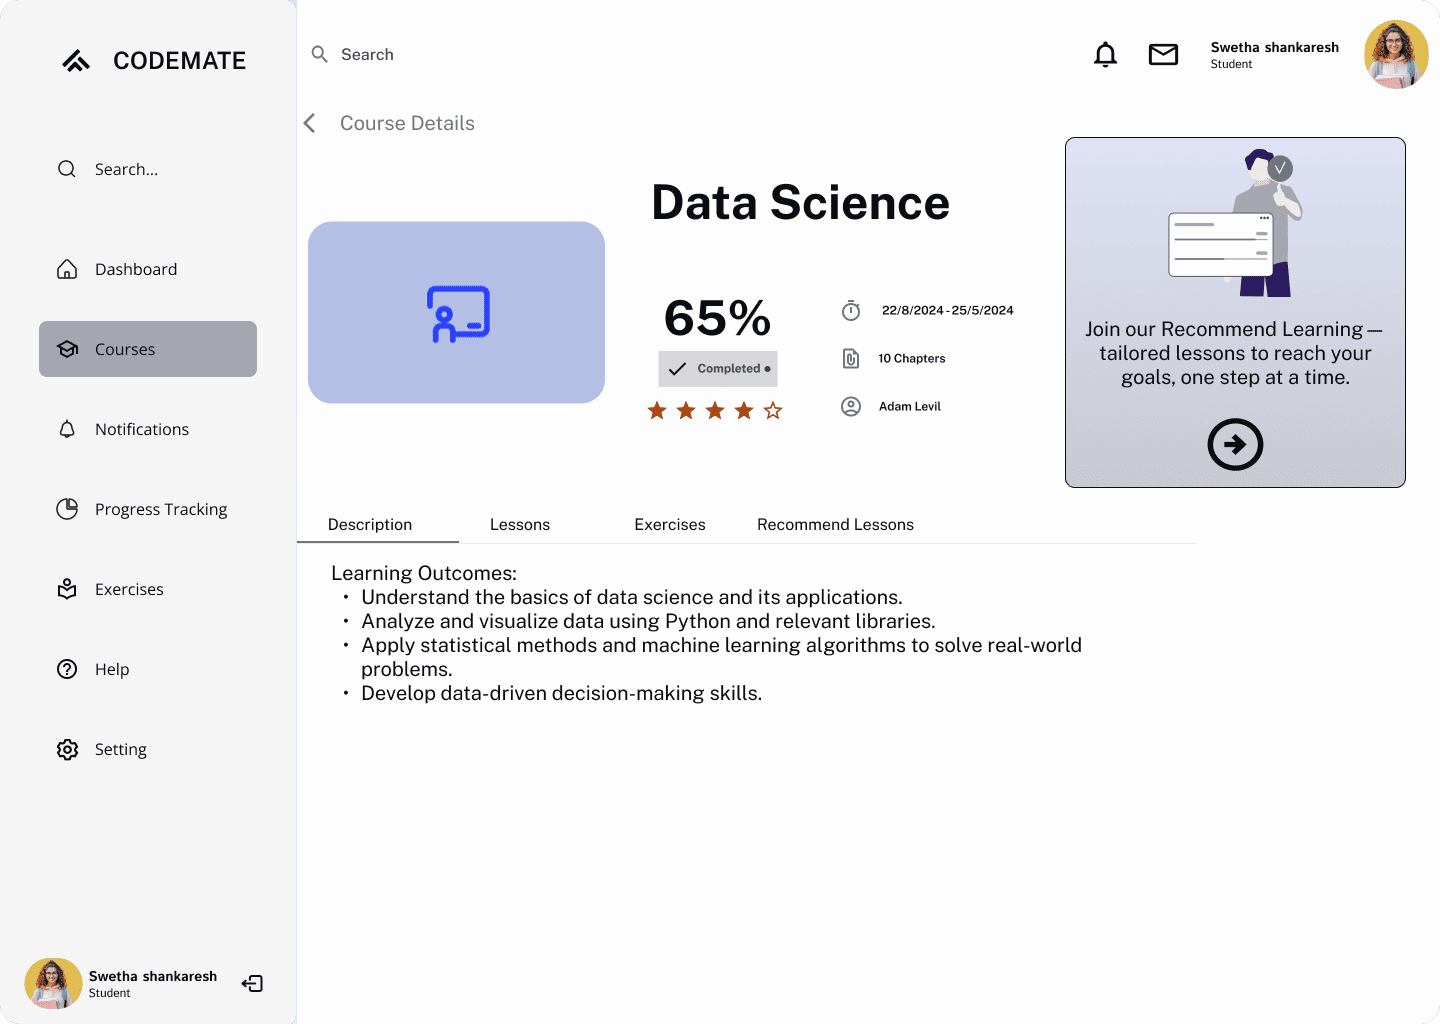
\includegraphics[width=0.7\linewidth]{Images/figmaDesign/Detailed Course Page - Description.png}
    \caption{Detailed Course Screen - Description}
    \label{fig:enter-label}
\end{figure}
Field Description chứa thông tin liên quan đến mô tả khóa học và đầu ra môn học do giảng viên cung cấp.
\begin{figure}[H]
    \centering
    
\includegraphics[width=0.7\linewidth]{Images/figmaDesign/Detailed Course Page - Lessons.png}
    \caption{Detailed Course Page - Lessons}
    \label{fig:enter-label}
\end{figure}
Field Lessons chứa các lessons được chia bởi giảng viên. Mỗi lesson được hiển thị với thông tin: \textbf{\textit{Tên lesson và Số tài liệu tham khảo được giảng viên đăng tải}}
\begin{figure}[H]
    \centering
    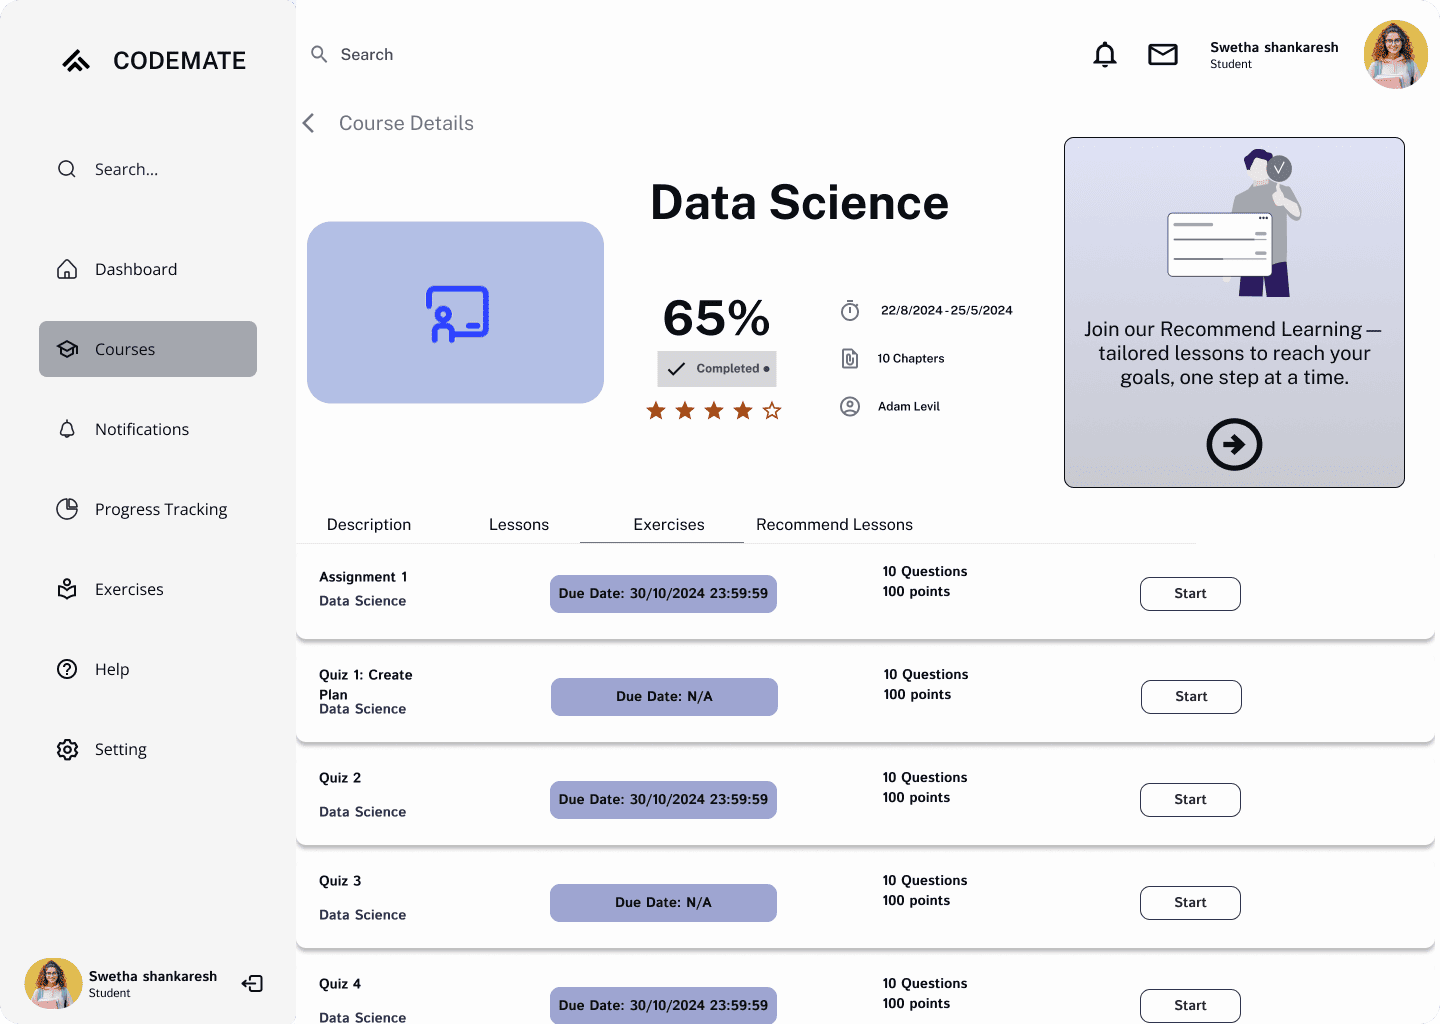
\includegraphics[width=0.7\linewidth]{Images/figmaDesign/Detailed Course Page - Exercises.png}
    \caption{Detailed Course Page - Exercises}
    \label{fig:enter-label}
\end{figure}
Field Exercises chứa các bài Quiz/Assignment do giảng viên hoặc hệ thống cung cấp hỗ trợ cho lesson/khóa học đó. 
\begin{figure}[H]
    \centering
    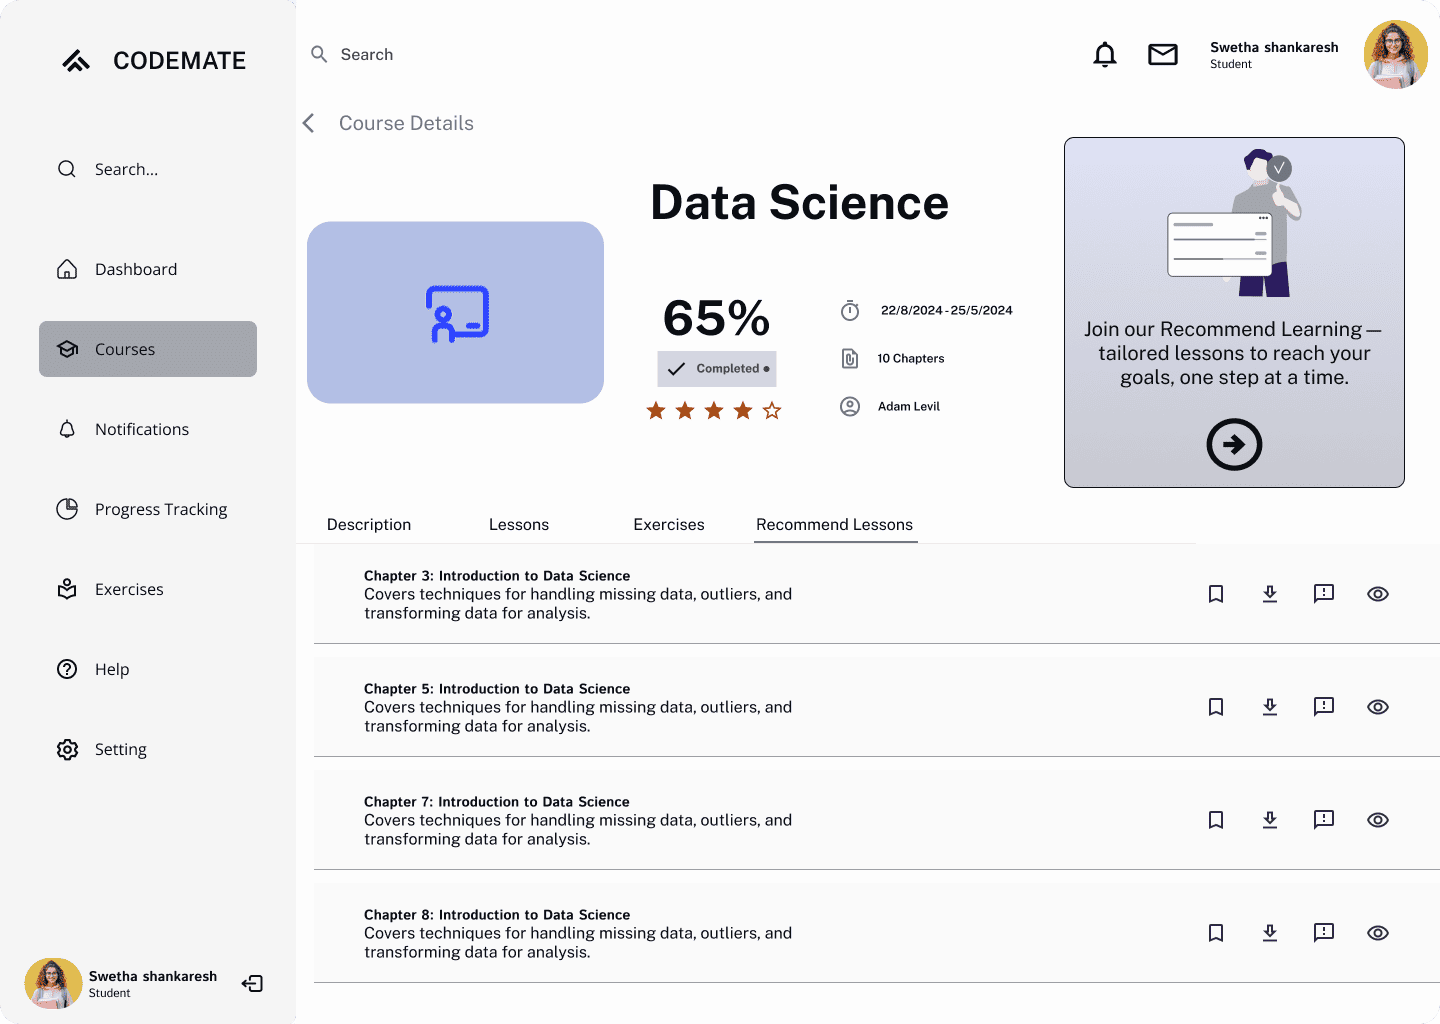
\includegraphics[width=0.7\linewidth]{Images/figmaDesign/Detailed Course Page - Recommend Lessons.png}
    \caption{Detailed Course Page - Recommend Lessons}
    \label{fig:enter-label}
\end{figure}
Field Recommend Lessons Chứa các lessons mà hệ thống đã đề xuất cho sinh viên. 
\subsubsection{Define Goal Modal}
\begin{figure}[H]
    \centering
    
\includegraphics[width=0.7\linewidth]{Images/figmaDesign/Get Goals Modal.png}
    \caption{Modal để lấy mục tiêu của sinh viên}
    \label{fig:enter-label}
\end{figure}
Sinh viên có thể cung cấp mục tiêu học tập của mình thông qua modal ở trang chi tiết khóa học
\subsubsection{Modules}
Sau khi chọn mục tiêu học tập và được hệ thống đề xuất lesson, sinh viên sẽ được truy cập vào lesson được đề xuất với giao diện chi tiết lesson như sau: 
\begin{figure}[H]
    \centering
    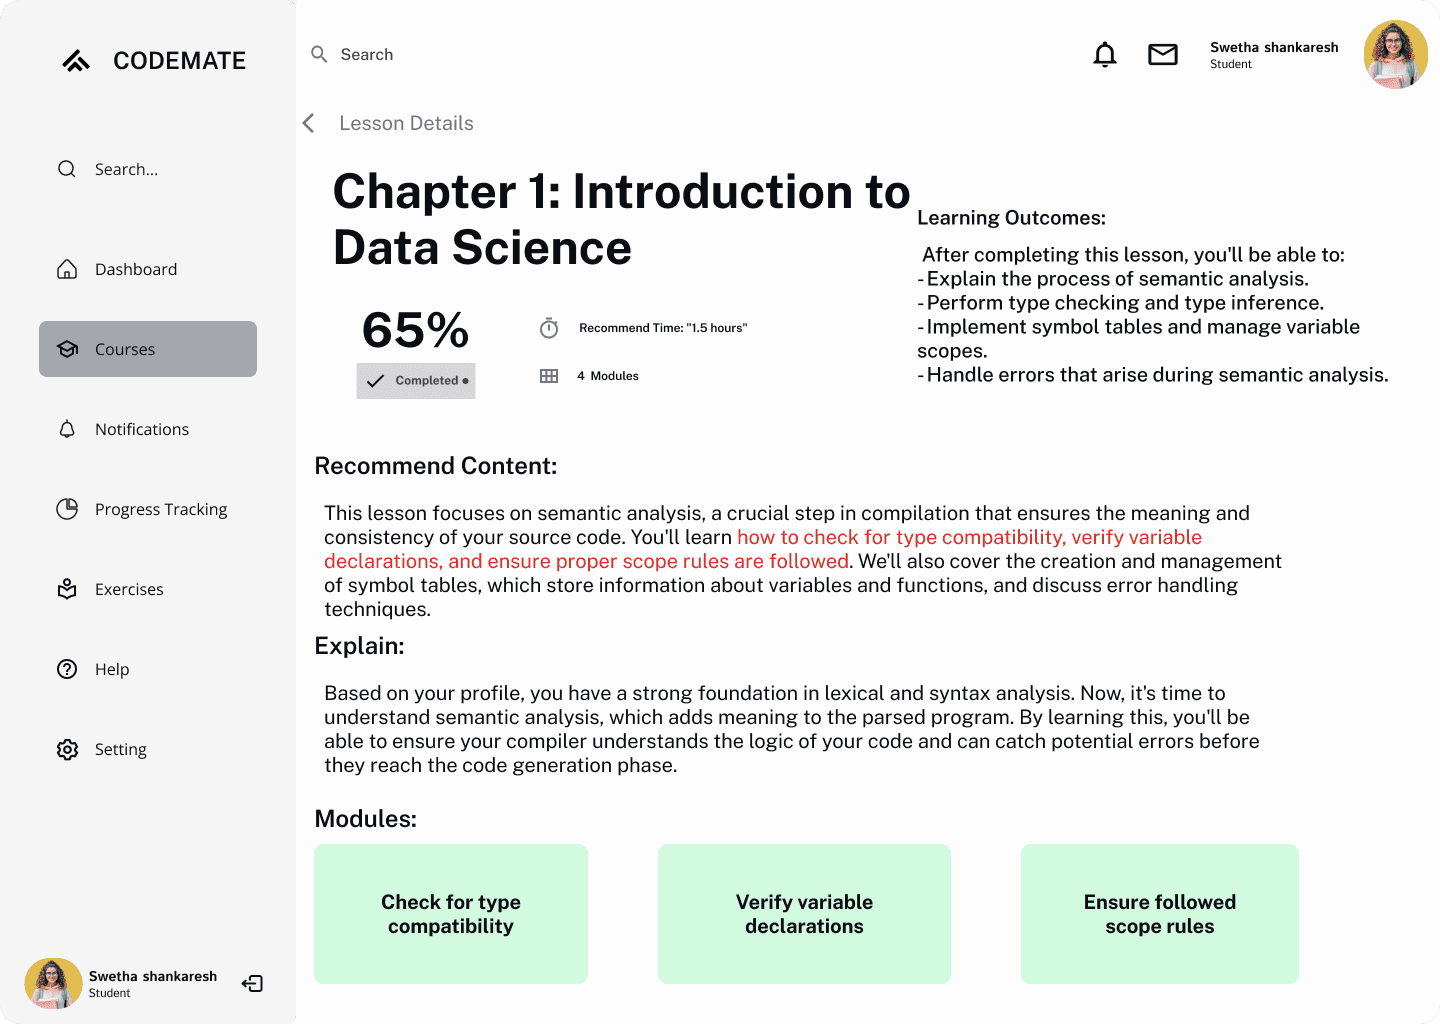
\includegraphics[scale=0.3]{Images/figmaDesign/Detailed Lesson Page.png}
    \caption{Chi tiết Lesson}
    \label{fig:enter-label}
\end{figure}
Lesson đề xuất sẽ cung cấp đầy đủ thông tin về \textbf{\textit{Learning Objectives, Recommend Content, Lời giải thích cho sự đề xuất và các modules cần học}}
\subsubsection{Choices of Learning Styles}
\begin{figure}[H]
    \centering
    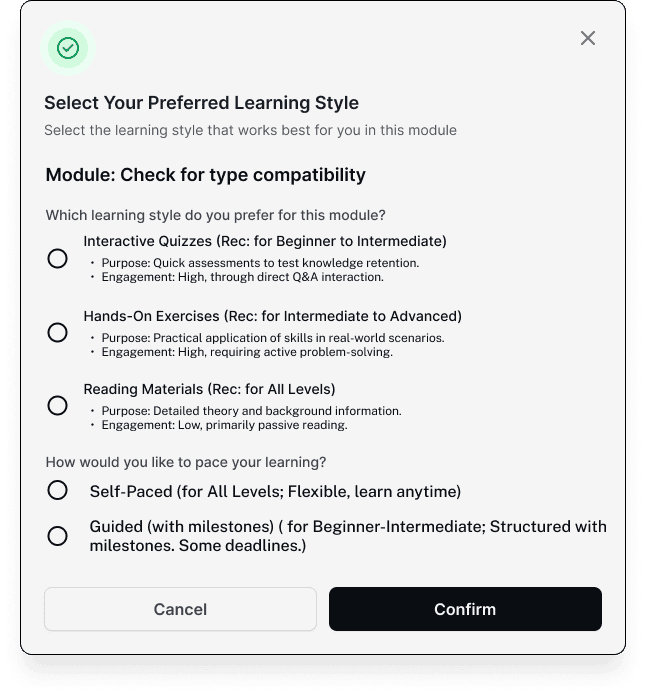
\includegraphics[scale=0.3]{Images/figmaDesign/Get Learning Style Modal.png}
    \caption{Modal cho phép sinh viên lựa chọn kiểu học phù hợp}
    \label{fig:enter-label}
\end{figure}
Sinh viên cung cấp thông tin về cách học mong muốn và tốc độ phù hợp với bản thân ở Modal này để quyết định cách học cho từng module
\begin{figure}[H]
    \centering
    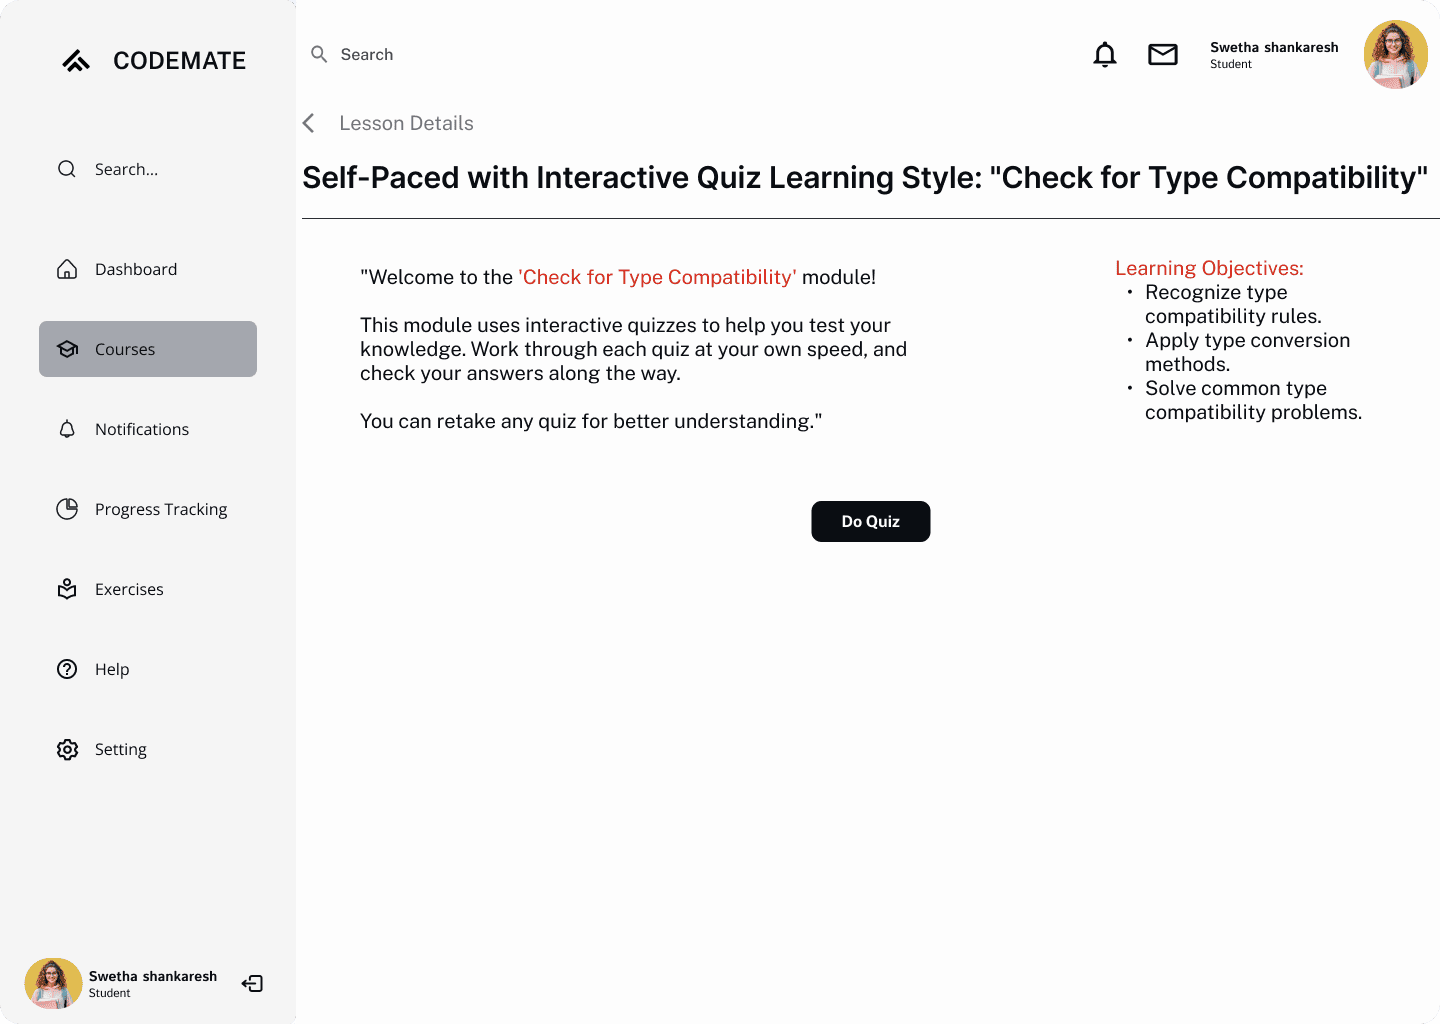
\includegraphics[scale=0.3]{Images/figmaDesign/Detailed Lesson Page - Self Pace Quiz.png}
    \caption{Giao diện khi sinh viên chọn học theo cách học làm Quiz với tiến độ tự do}
    \label{fig:enter-label}
\end{figure}
\begin{figure}[H]
    \centering
    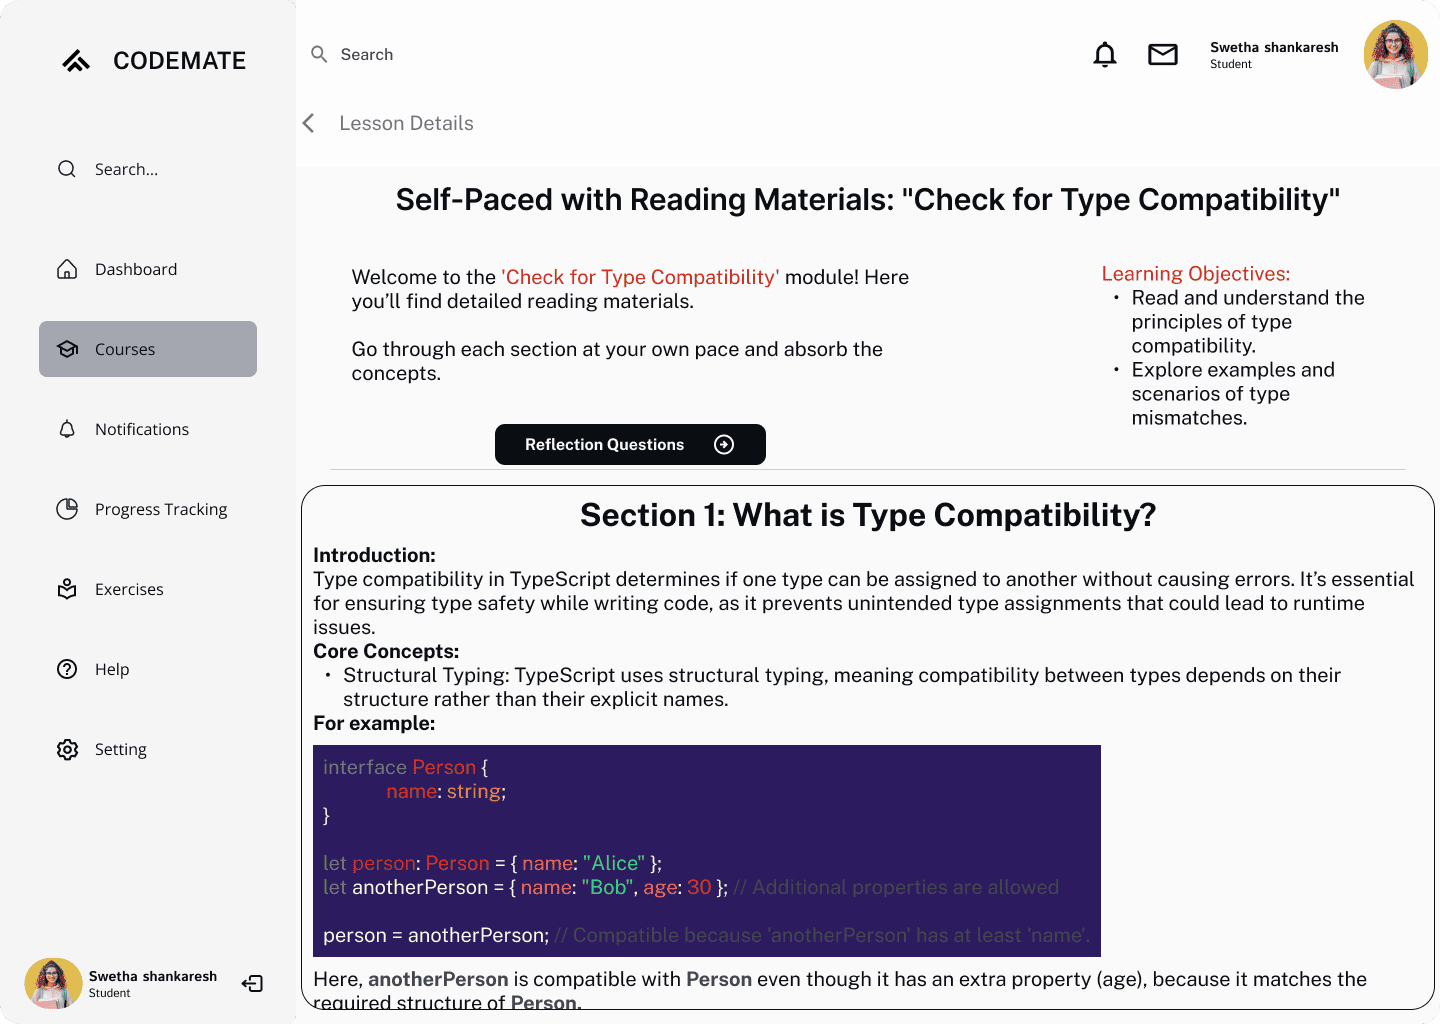
\includegraphics[scale=0.3]{Images/figmaDesign/Detailed Lesson Page - Self Pace Reading Material.png}
    \caption{Giao diện khi sinh viên chọn học theo cách học đọc tài liệu với tiến độ tự do}
    \label{fig:enter-label}
\end{figure}
\begin{figure}[H]
    \centering
    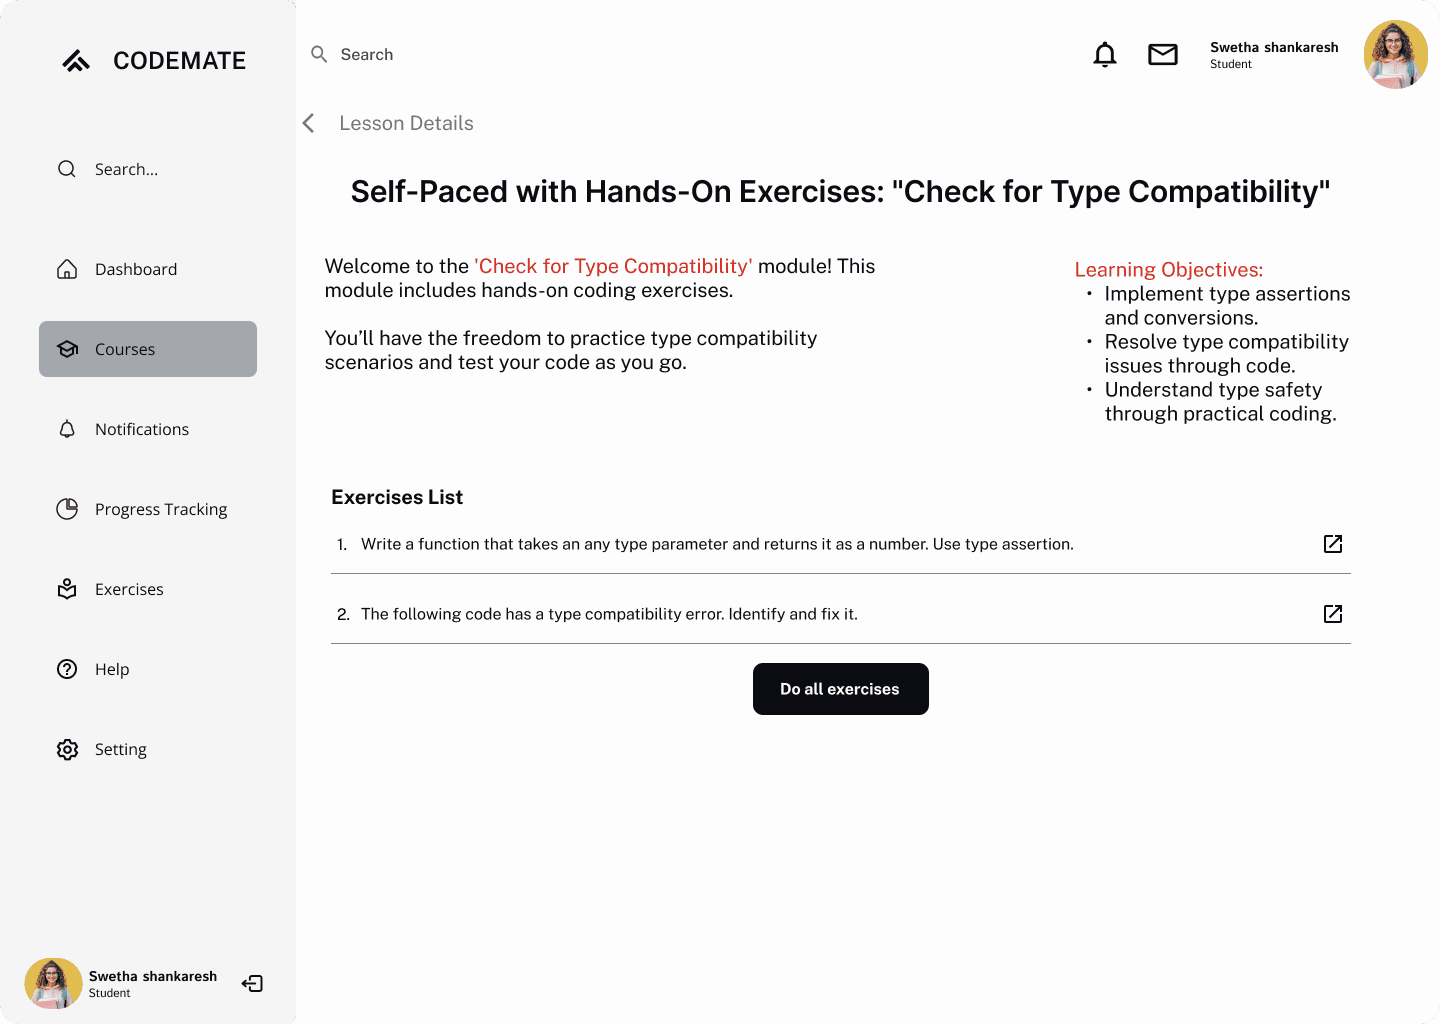
\includegraphics[scale=0.3]{Images/figmaDesign/Detailed Lesson Page - Self Pace Hands On Exercise.png}
    \caption{Giao diện khi sinh viên chọn học theo cách học làm bài tập Coding với tiến độ tự do}
    \label{fig:enter-label}
\end{figure}
\subsection{User Profile}
\subsubsection{Profile Information}
\begin{figure}[H]
    \centering
    \begin{subfigure}[b]{0.45\linewidth}
        \centering
        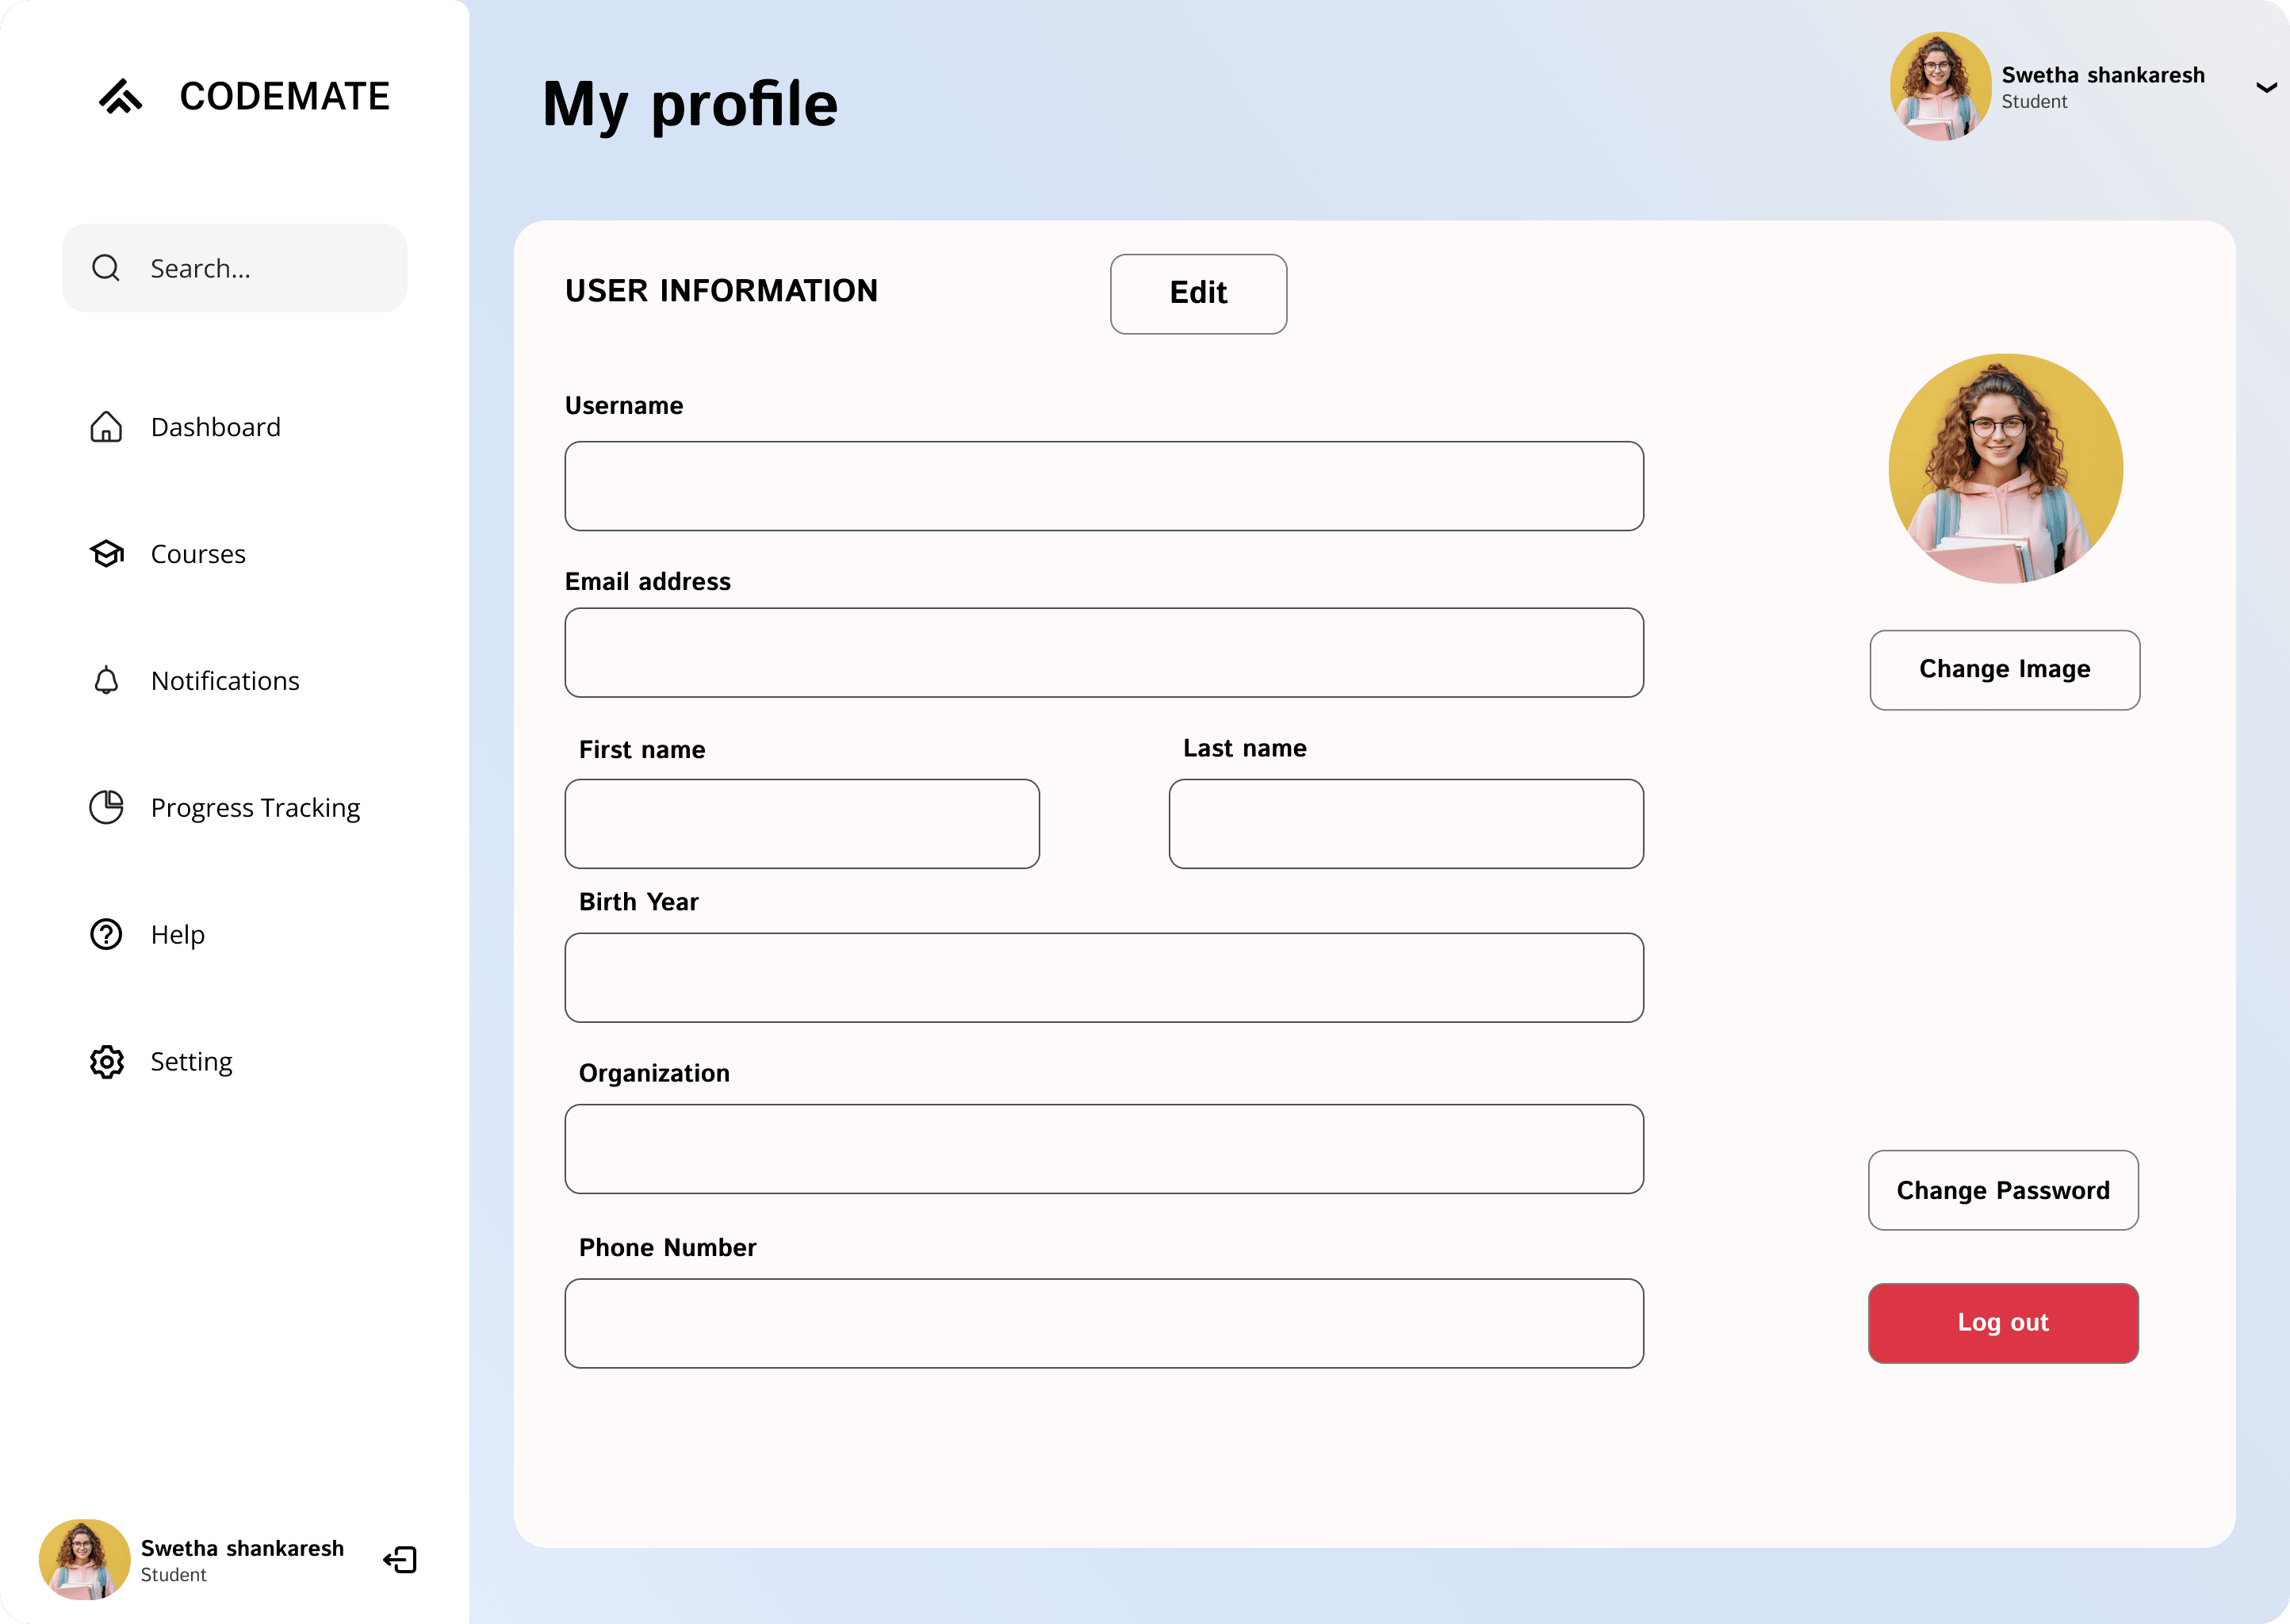
\includegraphics[width=\linewidth]{Images/Anh/UI_profile.png}
        \caption{Trang thông tin tài khoản}
        \label{fig:enter-label1}
    \end{subfigure}
    \hfill
    \begin{subfigure}[b]{0.45\linewidth}
        \centering
        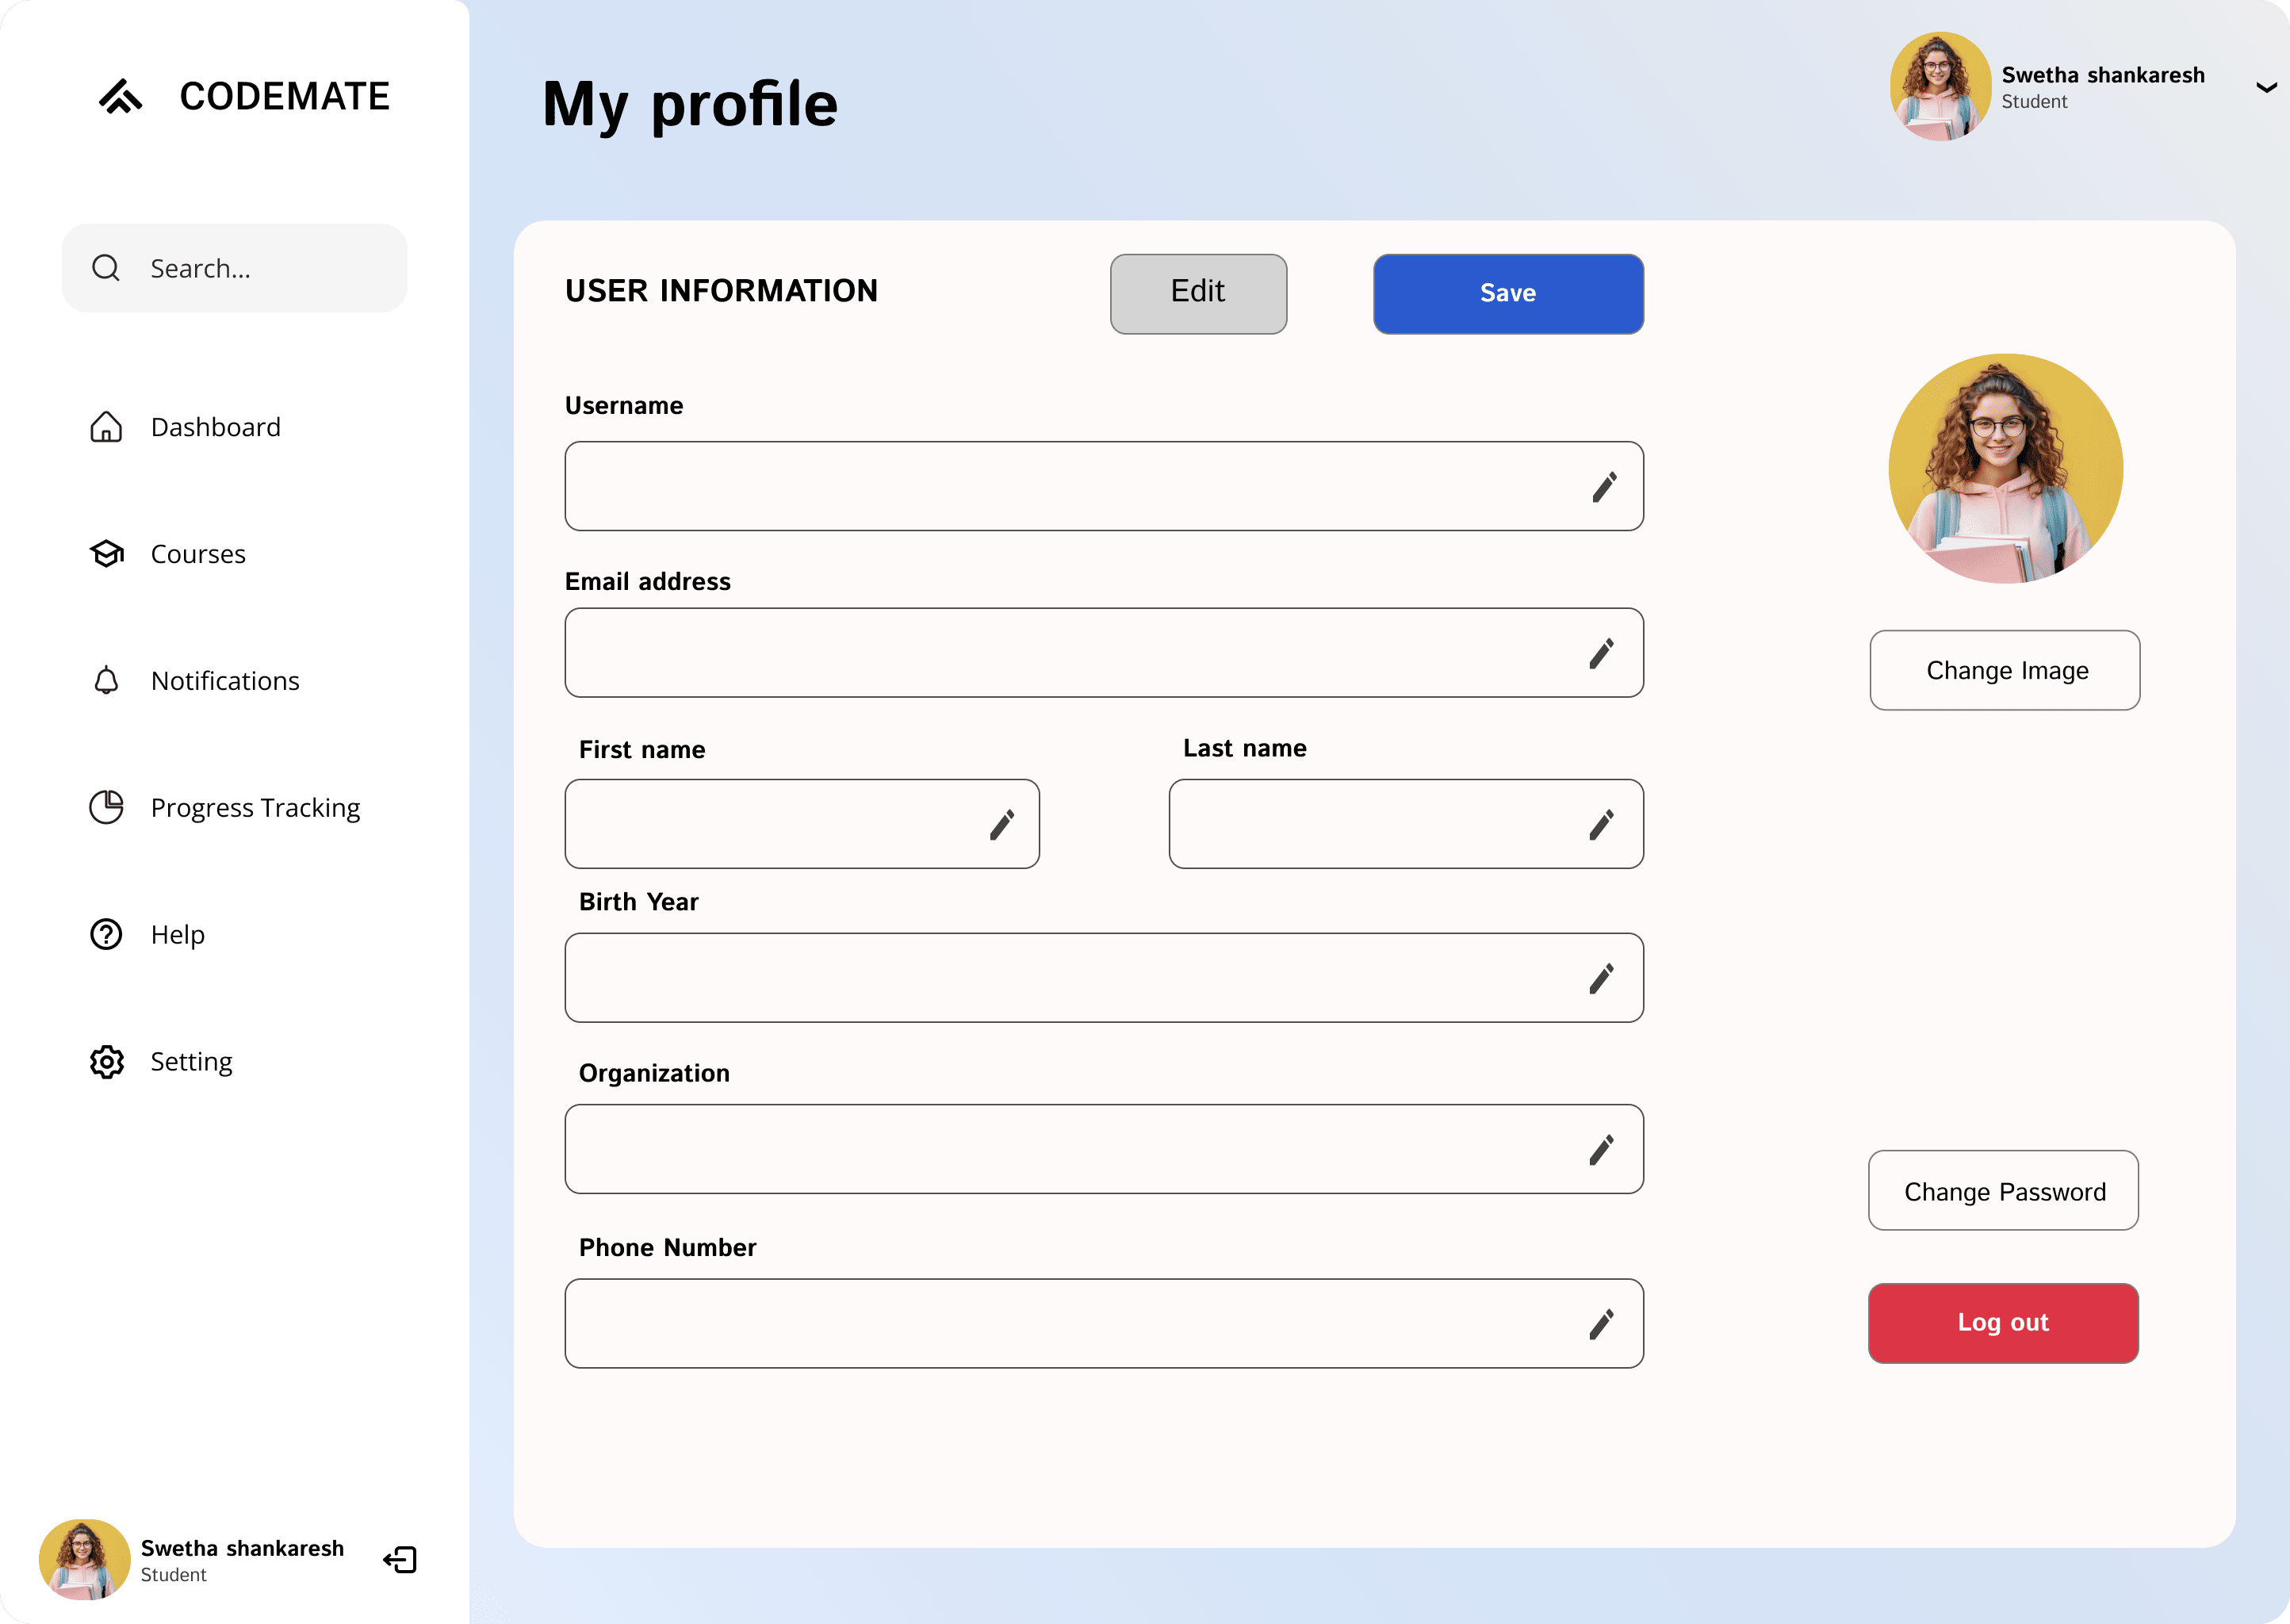
\includegraphics[width=\linewidth]{Images/Anh/UI_edit_profile.png}
        \caption{Chỉnh sửa thông tin tài khoản}
        \label{fig:enter-label2}
    \end{subfigure}
    \label{fig:enter-label}
\end{figure}
Trang "Thông tin tài khoản" cung cấp các trường thông tin cá nhân của người dùng bao gồm: Tên người dùng (Username), Địa chỉ email (Email address), Tên (First name), Họ (Last name), Năm sinh (Birth Year), Trường (Organization), và Số điện thoại (Phone Number). Người dùng có thể thay đổi hình ảnh đại diện bằng cách nhấp vào nút Change Image và cập nhật mật khẩu thông qua nút Change Password. Tất cả thông tin có thể được chỉnh sửa bằng cách nhấn vào nút Edit.
\subsubsection{Change Password, Avatar}
\begin{figure}[H]
    \centering
    \begin{subfigure}[b]{0.45\linewidth}
        \centering
        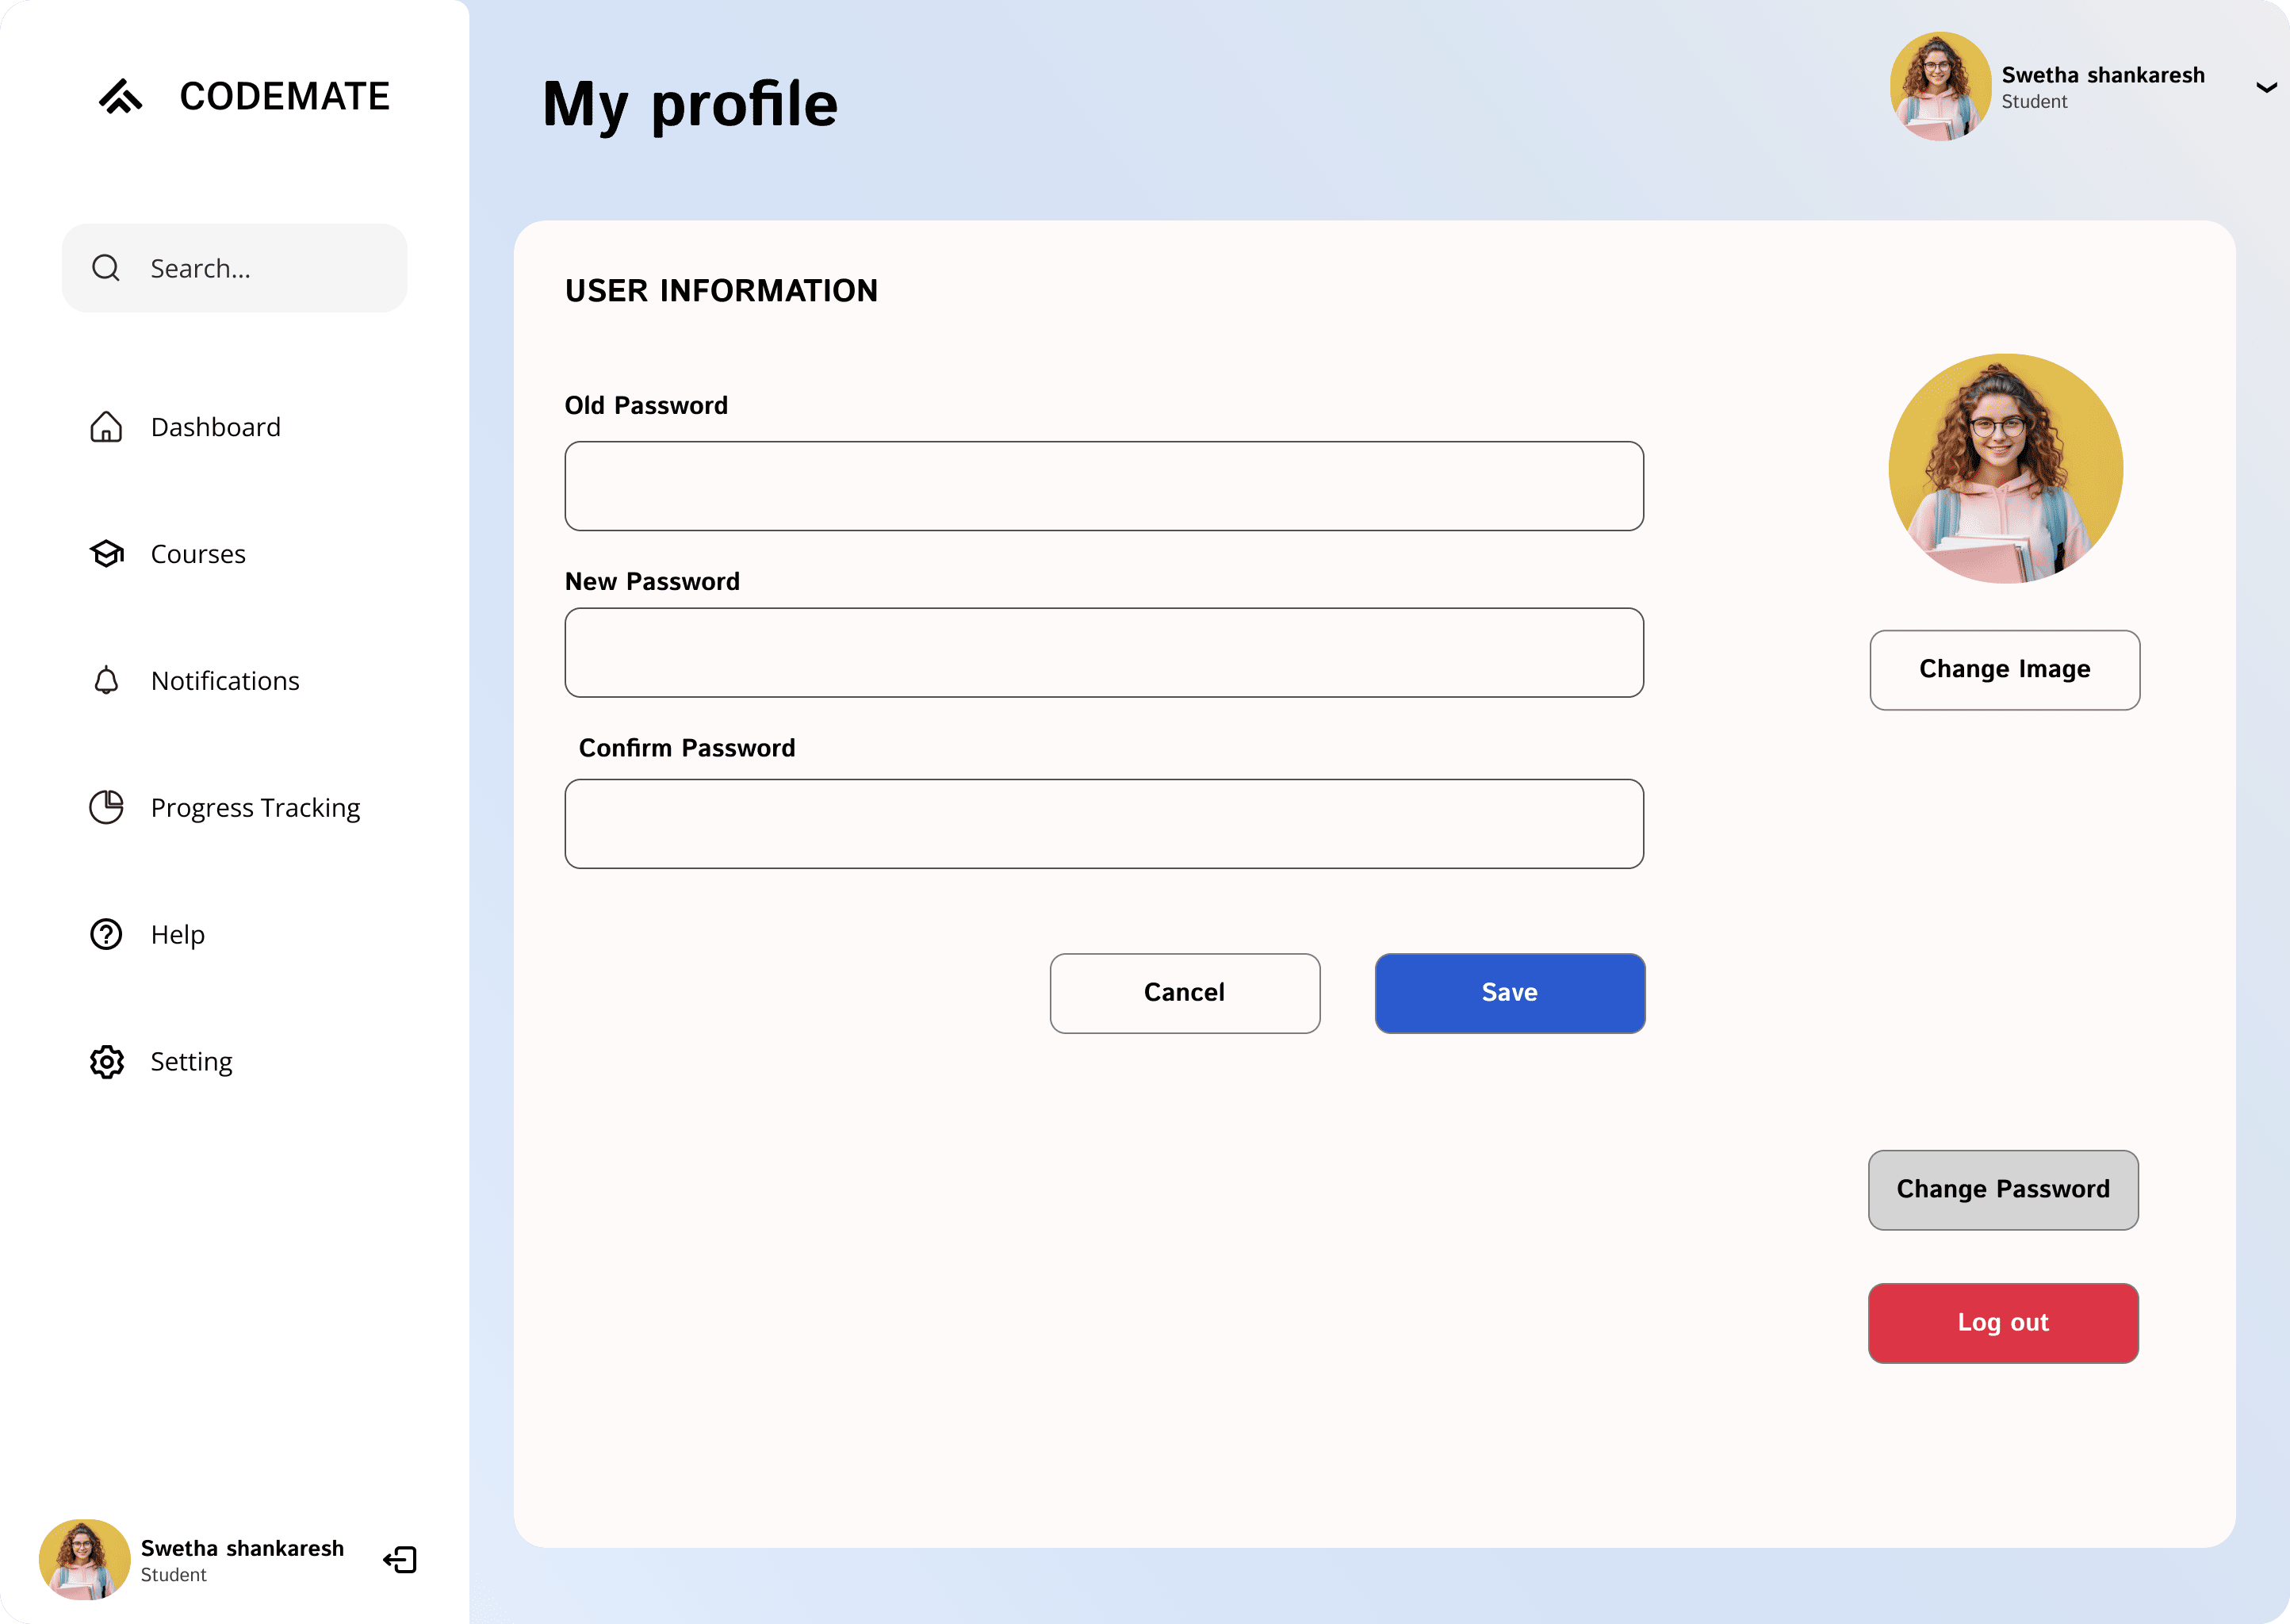
\includegraphics[width=\linewidth]{Images/Anh/UI_change_pass.png}
        \caption{Thay đổi mật khẩu}
        \label{fig:enter-label1}
    \end{subfigure}
    \hfill
    \begin{subfigure}[b]{0.45\linewidth}
        \centering
        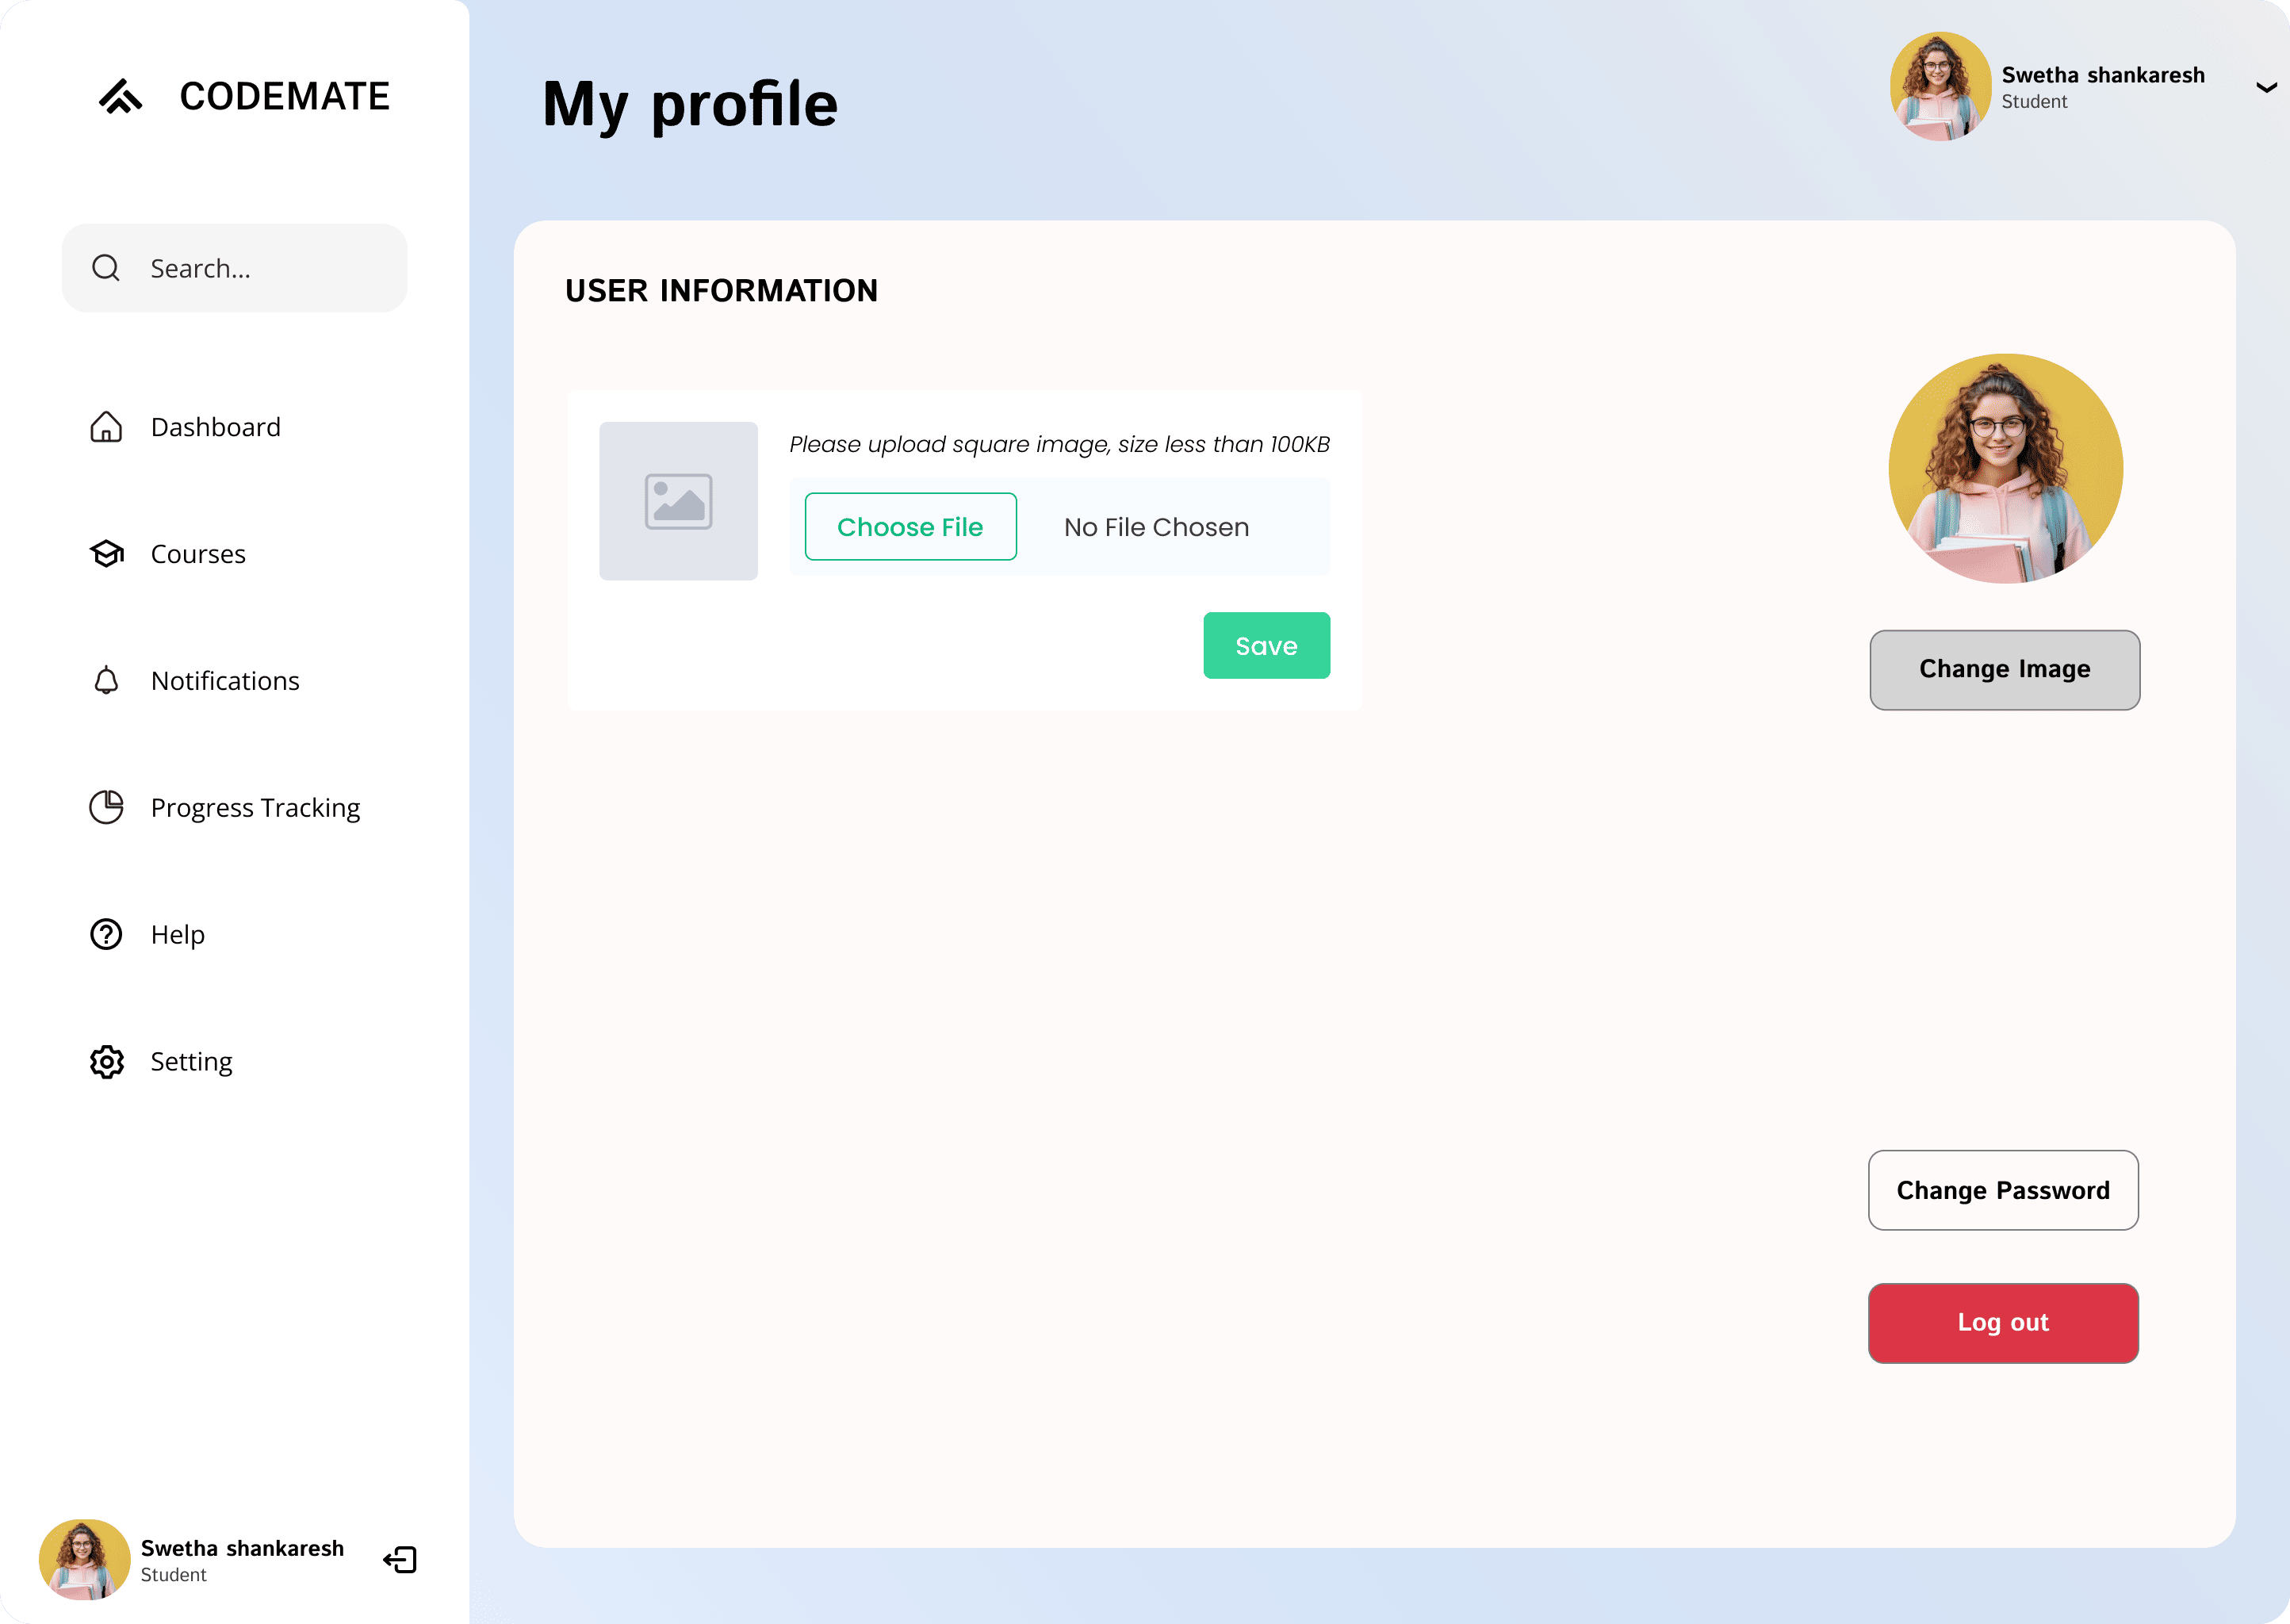
\includegraphics[width=\linewidth]{Images/Anh/UI_change_avatar.png}
        \caption{Thay đổi avatar}
        \label{fig:enter-label2}
    \end{subfigure}
    \label{fig:enter-label}
\end{figure}
Trang "Đổi mật khẩu" cho phép người dùng thay đổi mật khẩu bằng cách nhập mật khẩu hiện tại, mật khẩu mới, và xác nhận lại mật khẩu mới. Sau khi điền đầy đủ thông tin, người dùng nhấn nút "Đổi mật khẩu" để hoàn tất. Nếu có lỗi hoặc thành công, hệ thống sẽ hiển thị thông báo tương ứng. Trang "Đổi ảnh đại diện" cho phép người dùng tải lên ảnh mới từ thiết bị của mình và nhấn "Lưu thay đổi" để cập nhật ảnh đại diện.
\subsection{Dashboard Screen}
\begin{figure}[H]
    \centering
    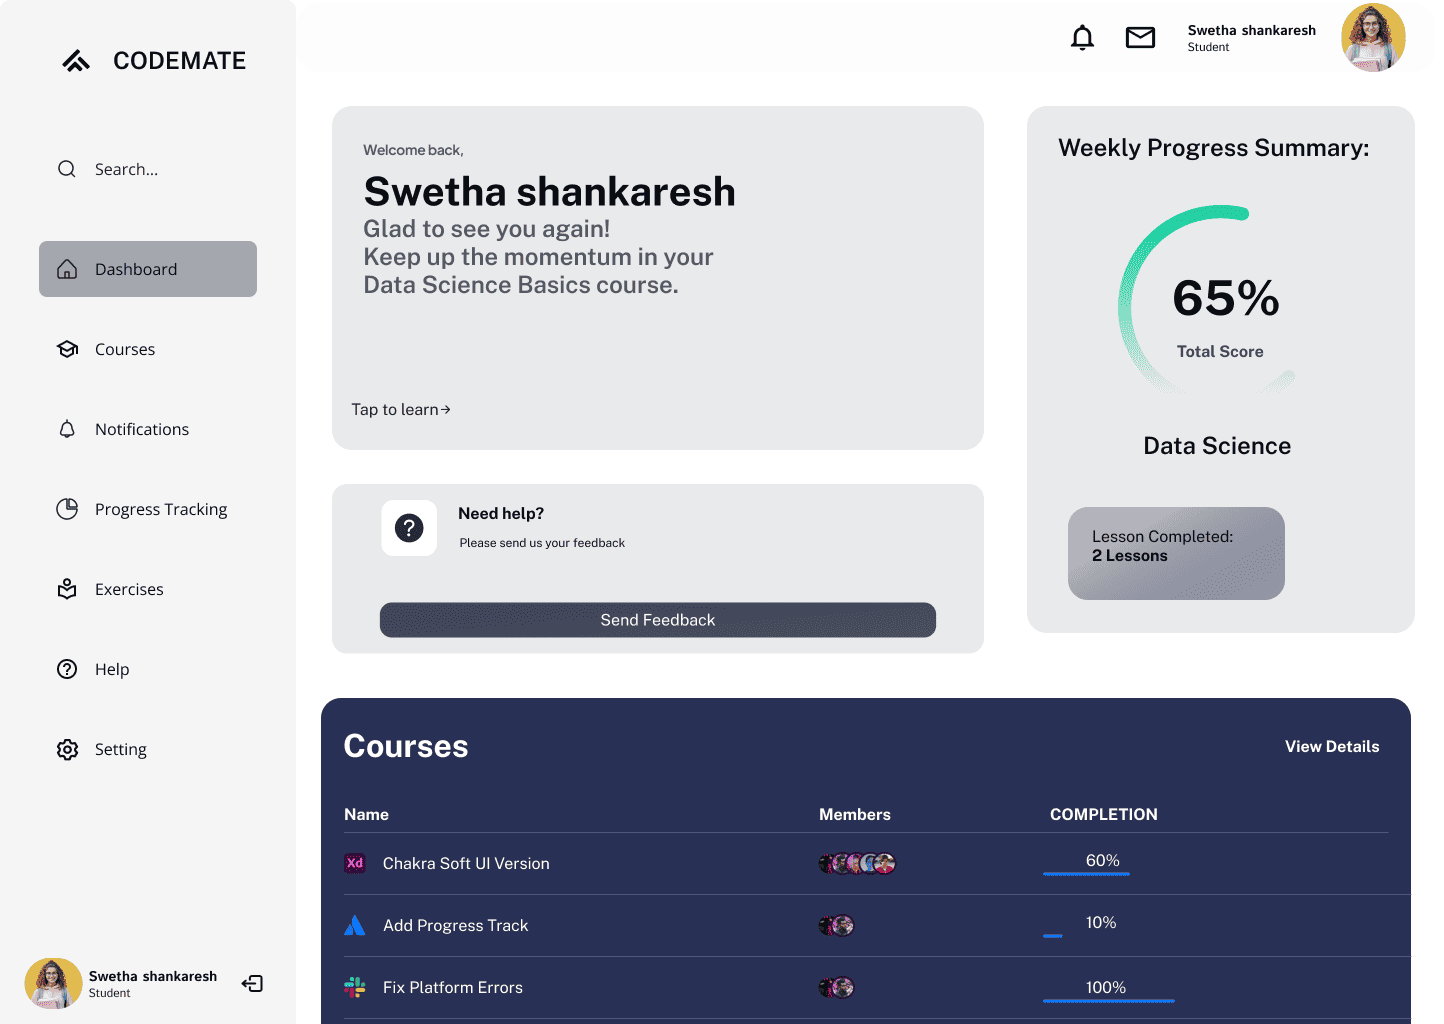
\includegraphics[width=1\linewidth]{Images/figmaDesign/Dashboard - Student.png}
    \caption{Dashboard - Student}
    \label{fig:enter-label}
\end{figure}
Trang Dashboard của sinh viên, mô tả tóm tắt về các khóa học mà sinh viên đã và đang tham gia và một số thông tin về khóa học vừa học ở lần truy cập gần nhất.
\subsection{Exercise Practice}
\subsubsection{Code Exercise}
\begin{figure}[H]
    \centering
    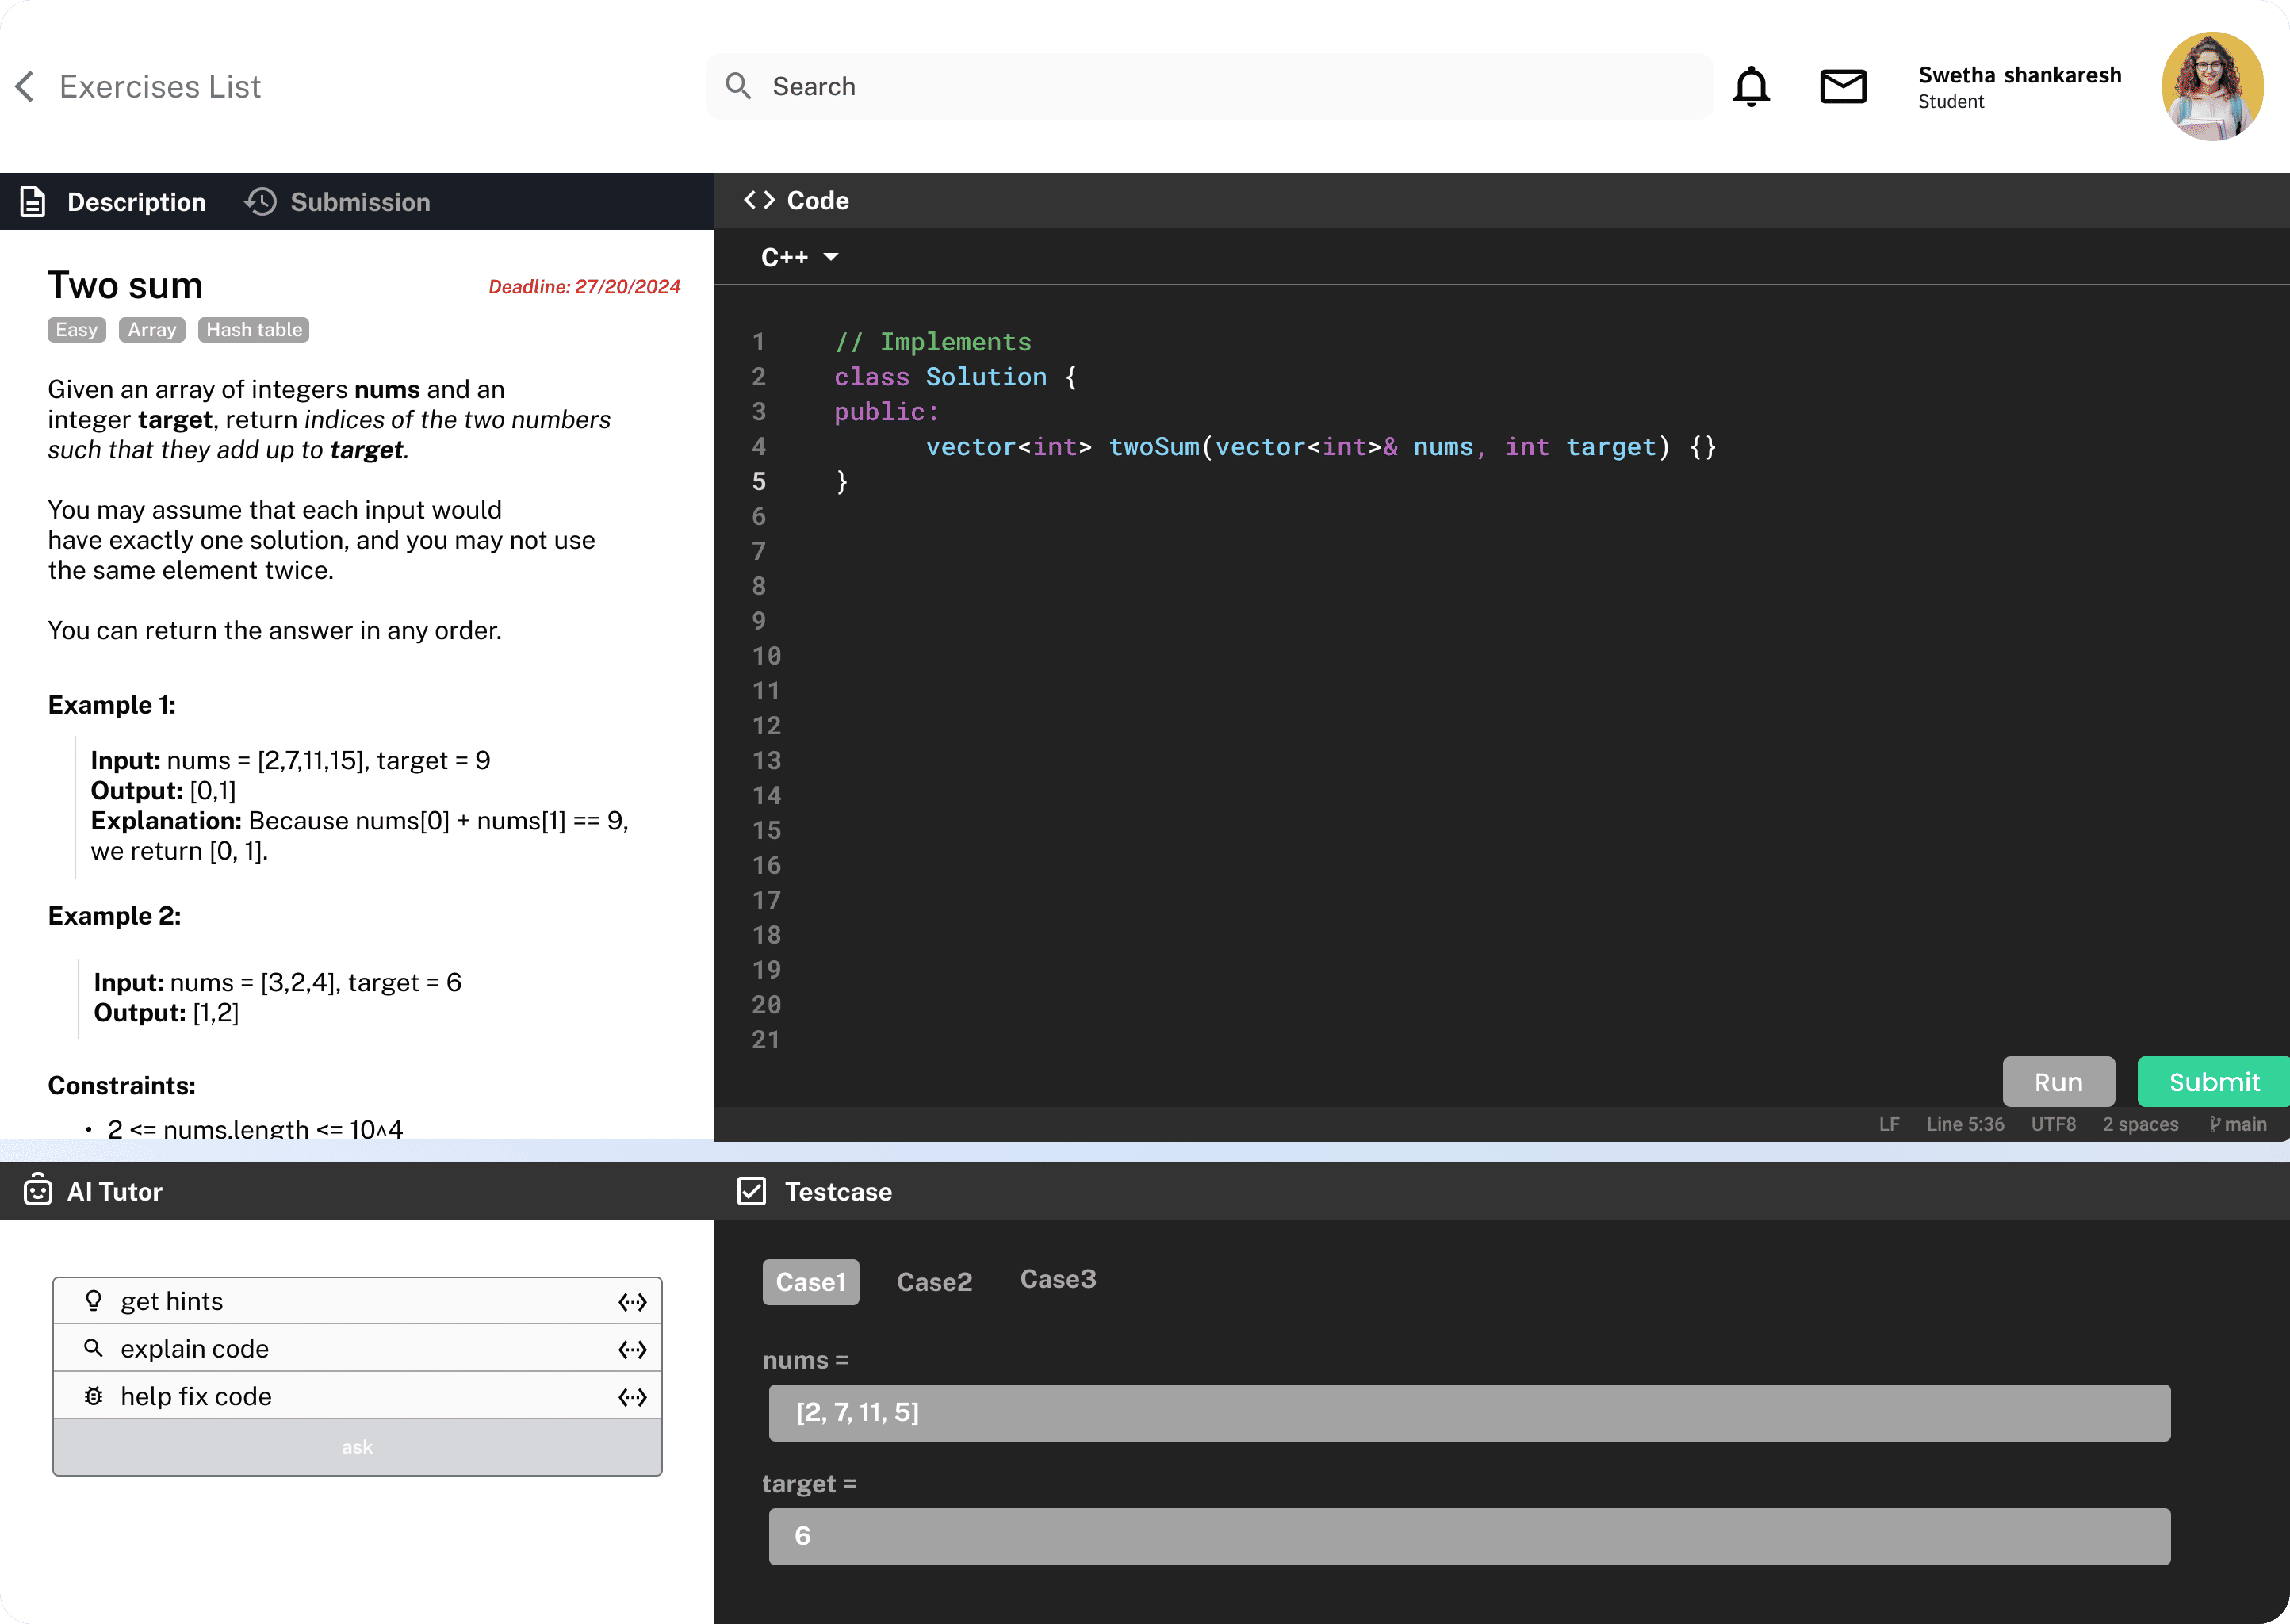
\includegraphics[width=0.7\linewidth]{Images/Anh/UI_practice_code.png}
    \caption{Giao diện thực hành code}
    \label{fig:enter-label}
\end{figure}
\begin{figure}[H]
    \centering
    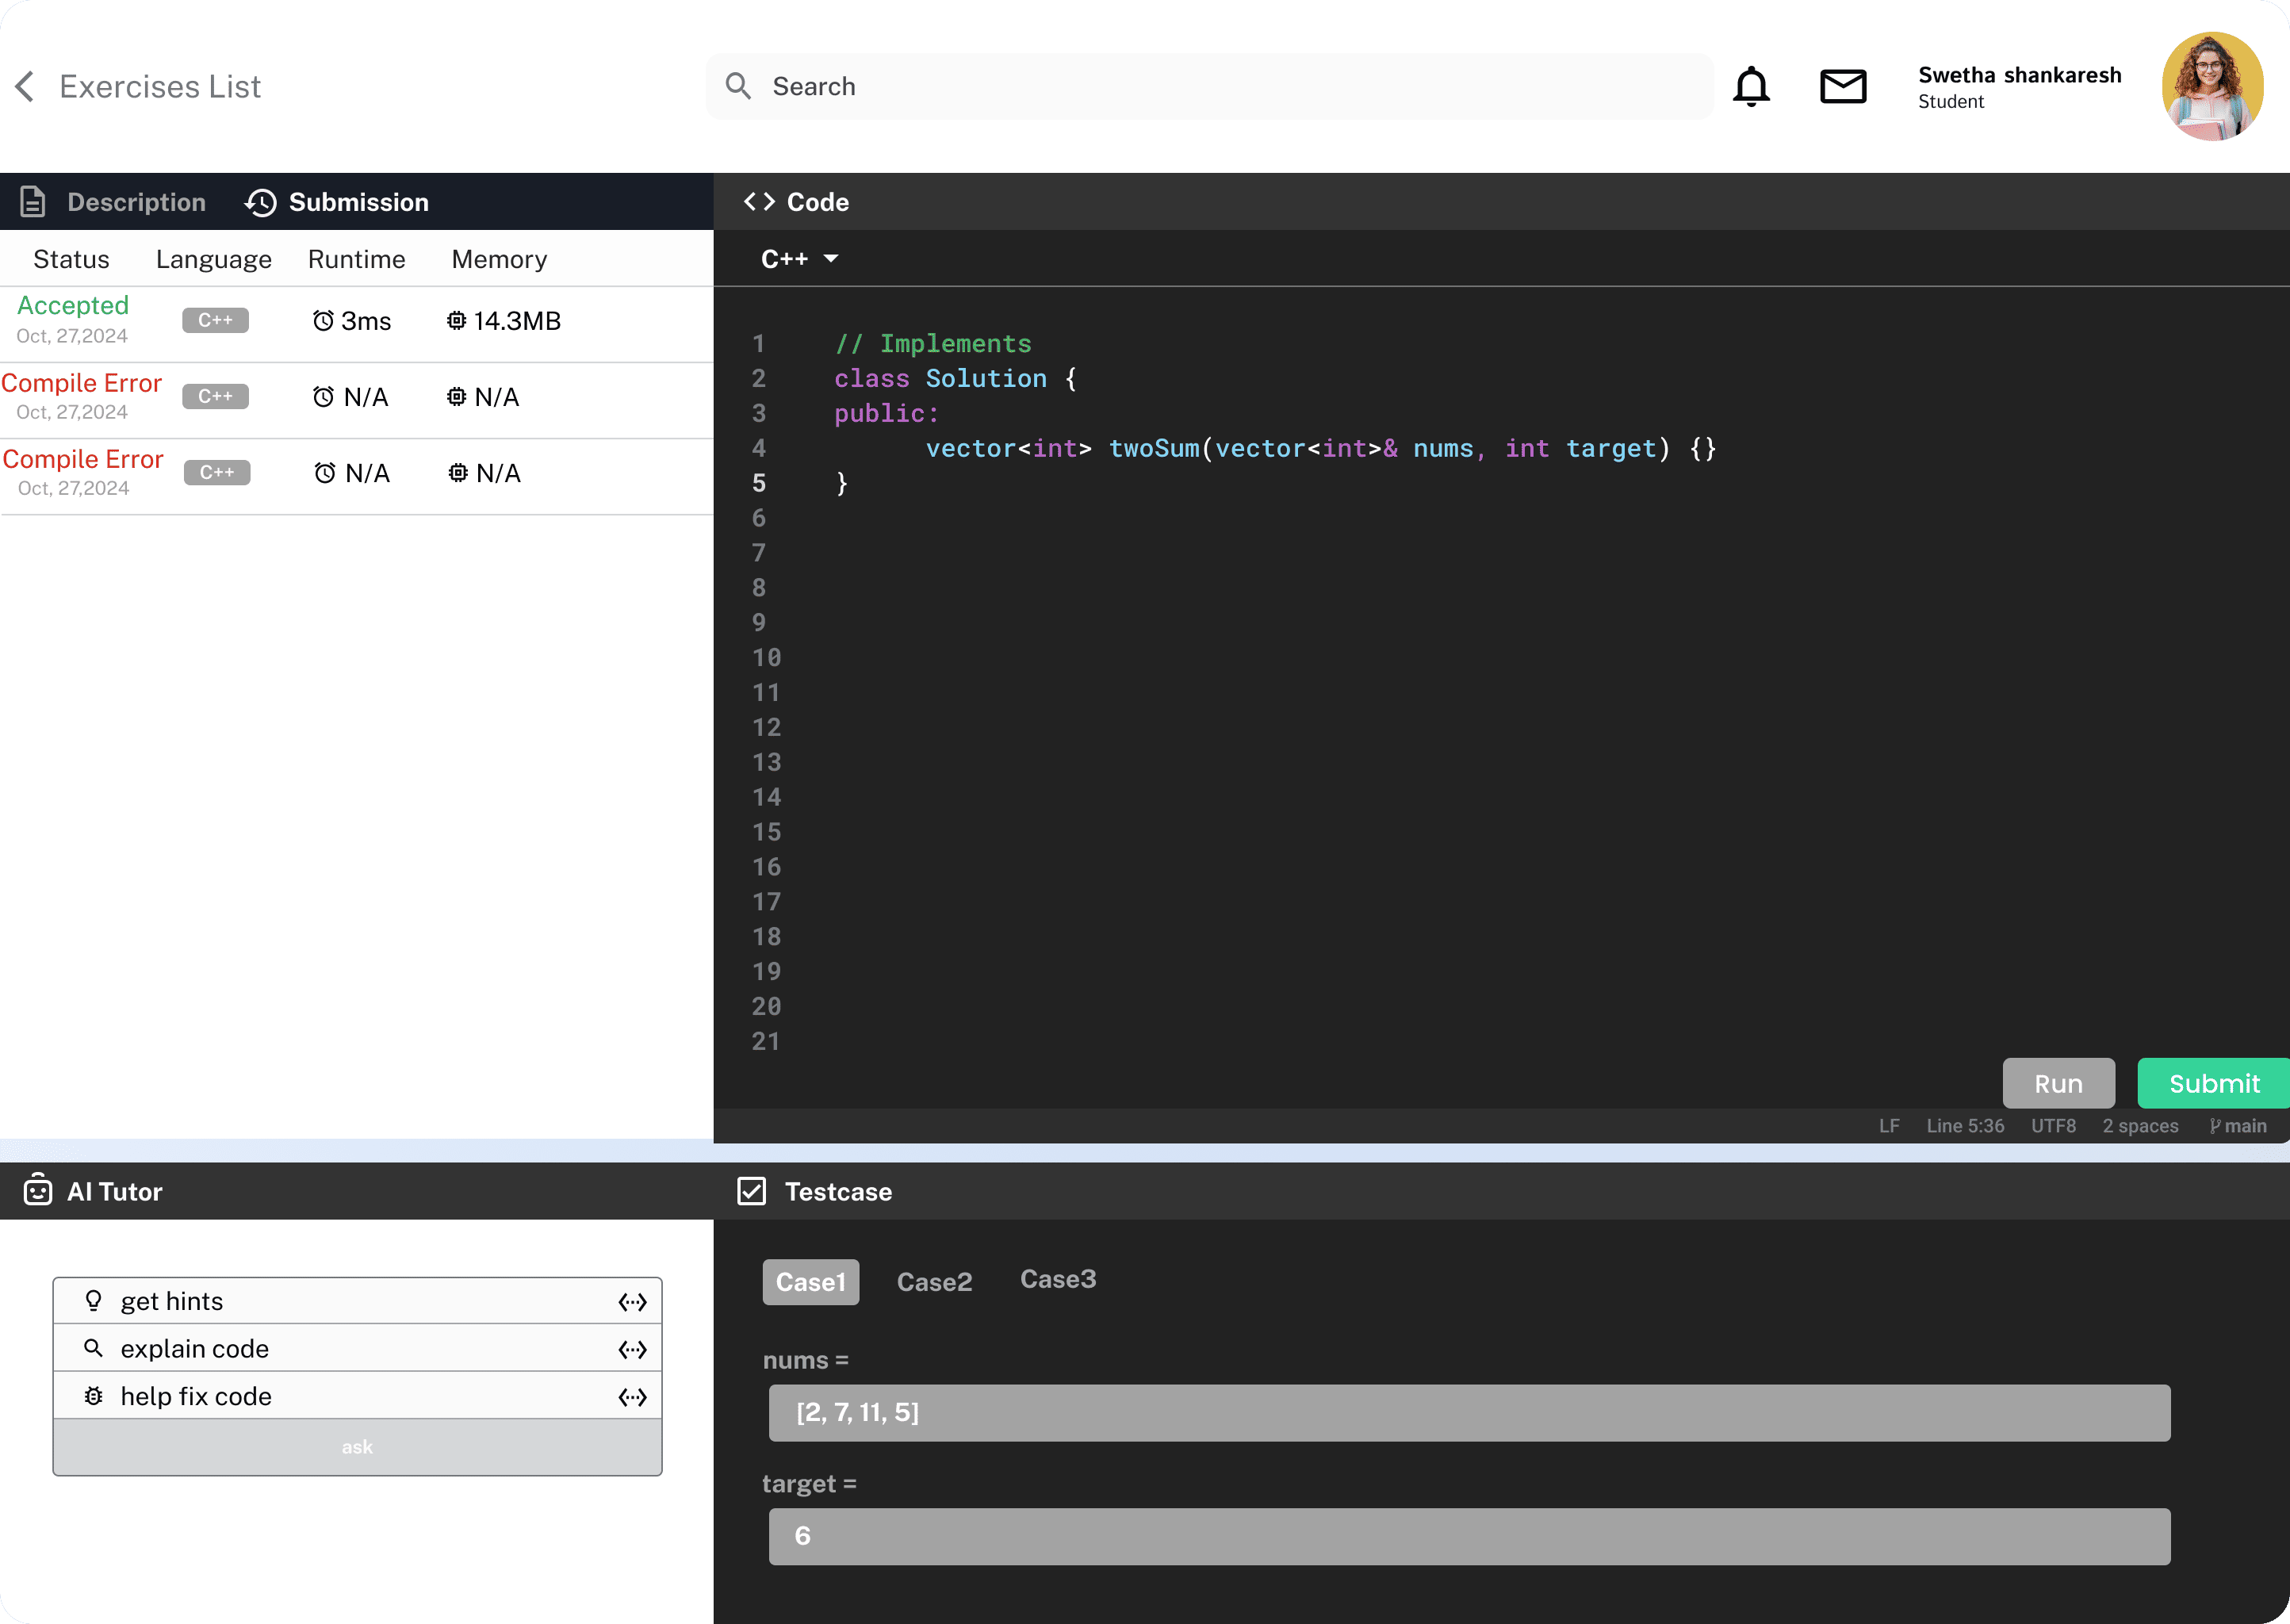
\includegraphics[width=0.7\linewidth]{Images/Anh/UI_Practice_submission.png}
    \caption{Lịch sử submission}
    \label{fig:enter-label}
\end{figure}
\subsection{AI Tutor}
Giao diện AI Tutor được thiết kế gồm ba chức năng chính như sau: cung cấp gợi ý (Get Hints), sửa lỗi (Fix Bug), và giải thích code (Explain Code). 
\begin{figure}[H]
    \centering
    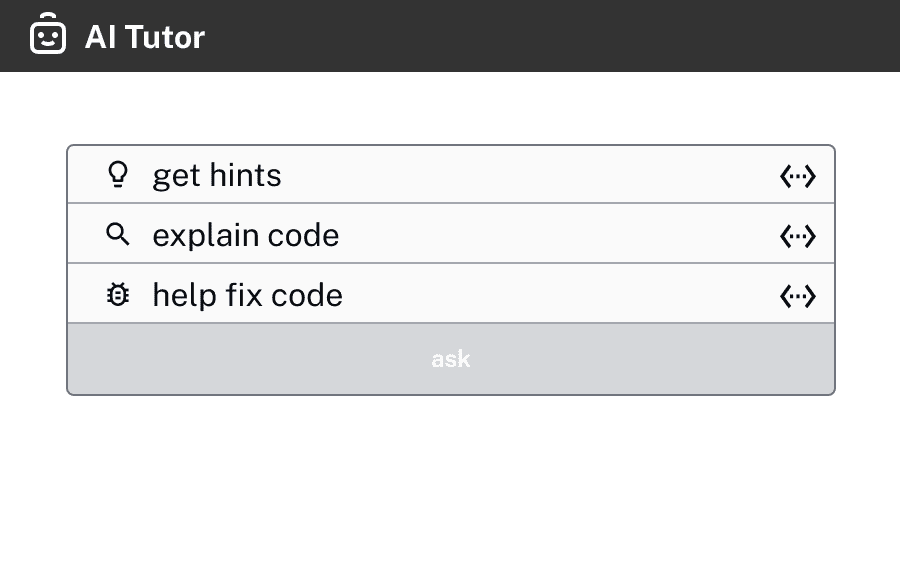
\includegraphics[width=0.7\linewidth]{Images/Anh/UI_AI_tutor.png}
    \caption{Các tính năng của AI Tutor}
    \label{fig:enter-label}
\end{figure}
Trong phần giải thích code, người dùng có thể chọn đoạn mã muốn hiểu rõ hơn; AI Tutor sẽ cung cấp giải thích tổng quát cho đoạn mã đó, và khi người dùng di chuột lên từng dòng, một popup sẽ hiển thị giải thích chi tiết cho từng dòng.
\begin{figure}[H]
    \centering
    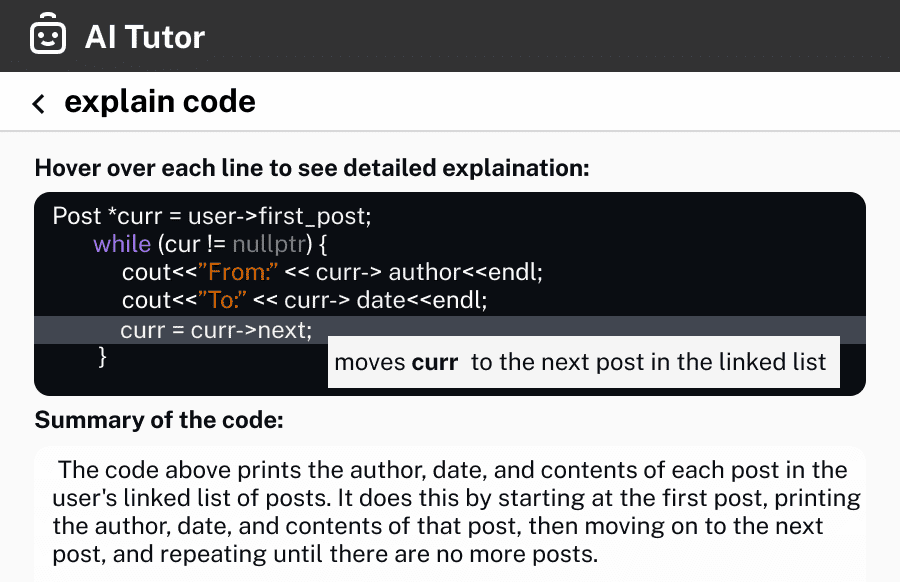
\includegraphics[width=0.7\linewidth]{Images/Anh/UI_AI_explain_code.png}
    \caption{Giải thích từng dòng code}
    \label{fig:enter-label}
\end{figure}
Đối với chức năng sửa lỗi, khi người dùng gặp lỗi trong quá trình compile code, AI Tutor sẽ phân tích và giải thích chi tiết nguyên nhân lỗi, đồng thời đề xuất cách khắc phục, giúp người dùng học hỏi từ lỗi sai của mình.
\begin{figure}[H]
    \centering
    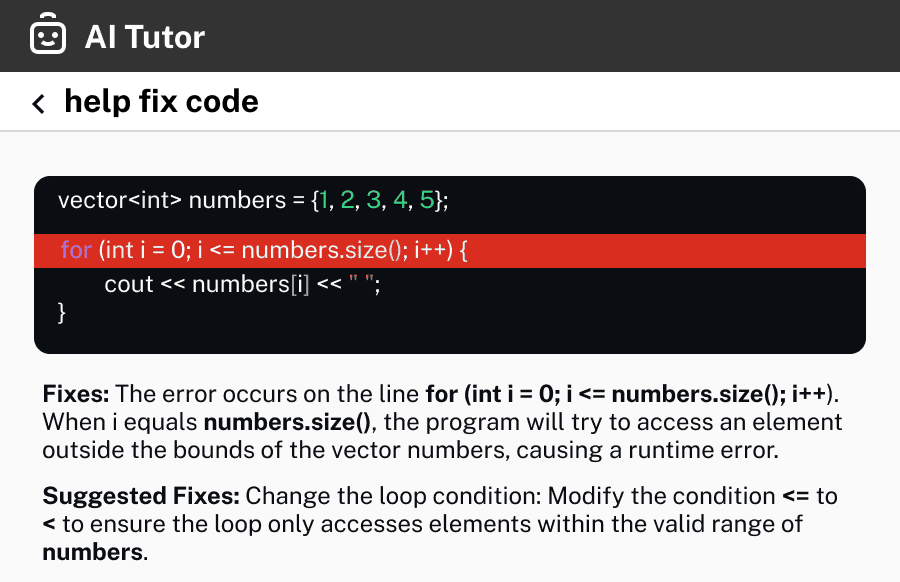
\includegraphics[width=0.7\linewidth]{Images/Anh/UI_help_fix_code.png}
    \caption{Hỗ trợ sửa lỗi}
    \label{fig:enter-label}
\end{figure}
Khi người dùng cần gợi ý cho bài tập, họ có thể nhấn nút "Get Hints" để nhận những hướng dẫn hữu ích; nếu chưa rõ, AI Tutor còn có thể đưa ra ví dụ minh họa giúp họ hiểu rõ hơn. 
\begin{figure}[H]
    \centering
    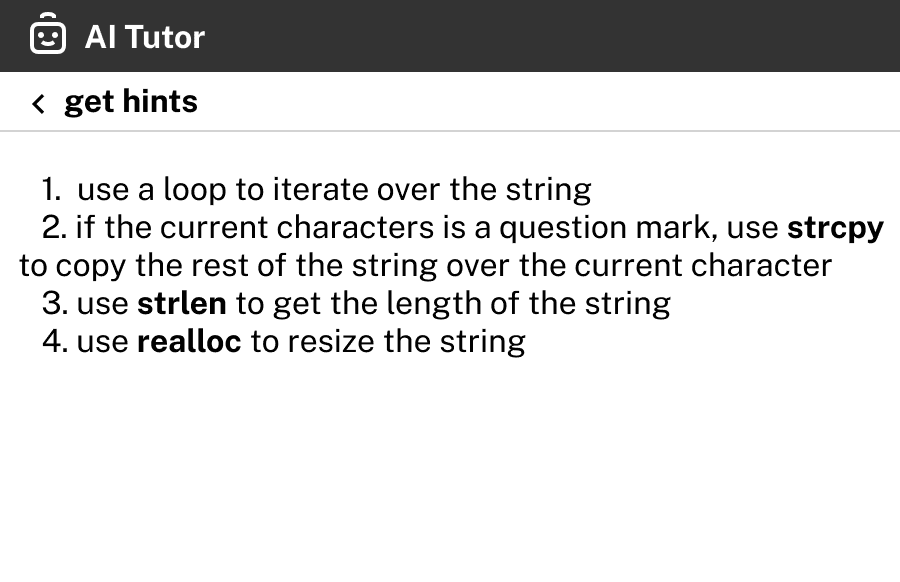
\includegraphics[width=0.7\linewidth]{Images/Anh/UI_AI_get_hints.png}
    \caption{Cung cấp gợi ý cho bài tập}
    \label{fig:enter-label}
\end{figure}
\subsection{Progress Tracking}
\begin{figure}[H]
    \centering
    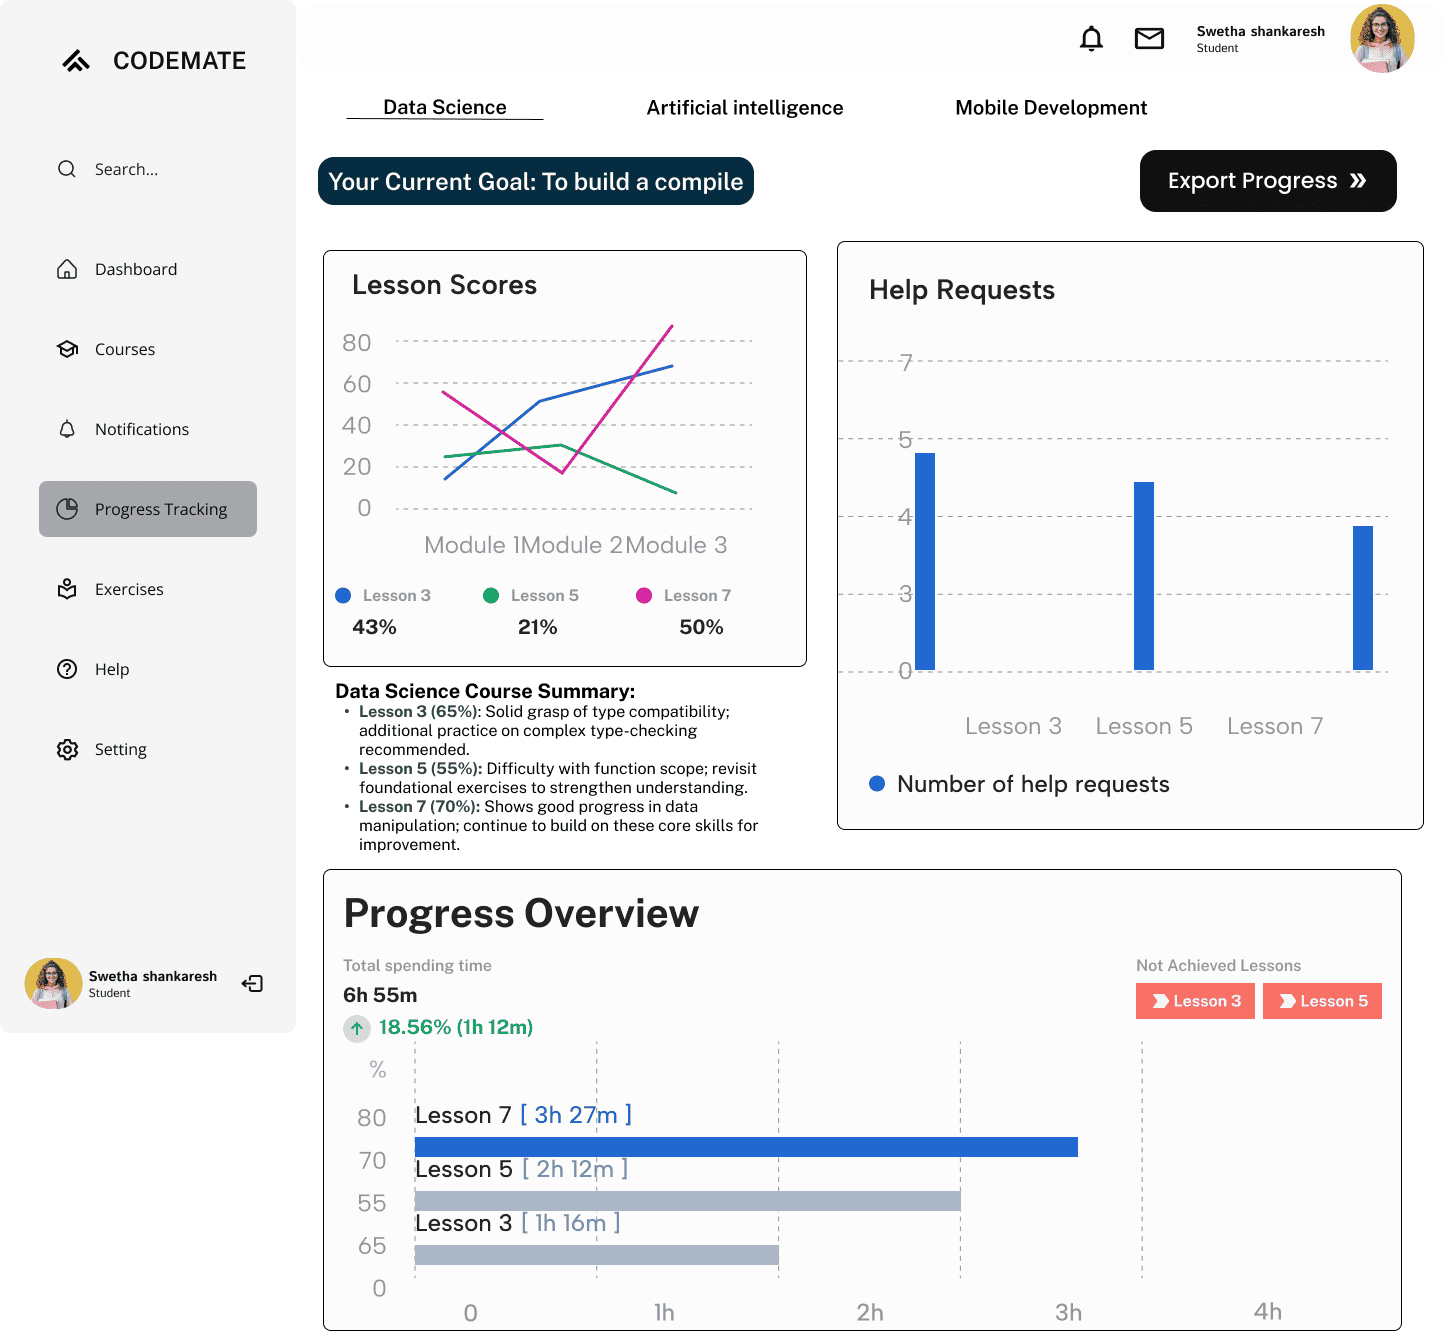
\includegraphics[width=1\linewidth]{Images/figmaDesign/Progress Tracking.png}
    \caption{Progress Tracking Page}
    \label{fig:enter-label}
\end{figure}
Trang Progress Tracking ghi lại tiến độ học tập của sinh viên theo từng môn học, bao gồm 3 biểu đồ chính: 
\begin{enumerate}
    \item \textbf{Biểu Đồ Đánh Giá Điểm Số Theo Lesson (Biểu đồ đường)}
    \begin{itemize}
        \item\textbf{X-Axis:} Tên module (1, 2, 3).
\item\textbf{Y-Axis:} Điểm số (từ 0 đến 100\%).
\item\textbf{Màu của đường biểu đồ:} Lesson(3,5,7)
\item\textbf{Đơn vị:} Phần trăm (\%).
\item\textbf{Ý Nghĩa:} Biểu đồ này cho phép sinh viên thấy tỷ lệ hoàn thành mục tiêu của từng module theo lesson và dễ dàng nhận ra lesson nào đạt hoặc chưa đạt yêu cầu, bị khó khăn ở module nào. 

    \end{itemize}
        \item \textbf{Biểu Đồ Theo Dõi Số Lượng Vấn Đề hoặc Yêu Cầu Trợ Giúp (Biểu đồ cột)}
    \begin{itemize}
        \item\textbf{X-Axis:} Tên lesson (1, 2, 3).
\item\textbf{Y-Axis:} Số lần sinh viên yêu cầu trợ giúp (Đếm số lần yêu cầu trợ giúp tới AI).
\item\textbf{Đơn vị:} Lần (Số lần hỏi).
\item\textbf{Ý Nghĩa:} Biểu đồ này ghi nhận độ khó của từng bài tập, giúp hệ thống nhận biết các phần cần được cải thiện hoặc các bài tập khó để review lại cho giáo viên hoặc sinh viên cần chú trọng học lại.
    \end{itemize}
            \item \textbf{Biểu Đồ Tổng Quan Tiến Độ Học (Progress Overview) (Biểu đồ cột)}
    \begin{itemize}
        \item\textbf{X-Axis:} Thời gian (Số giờ học).
\item\textbf{Y-Axis:} Tỷ lệ hoàn thành (\%) của lesson.
\item\textbf{Đơn vị:} Phần trăm (\%) hoàn thành lesson.
\item\textbf{Ý Nghĩa:} Cho thấy tiến độ tổng thể của sinh viên, giúp họ nhận ra tốc độ học của mình và đối chiếu với lộ trình học ban đầu.
    \end{itemize}
\end{enumerate}